%
% FH Technikum Wien
% !TEX encoding = UTF-8 Unicode
%
% Erstellung von Master- und Bachelorarbeiten an der FH Technikum Wien mit Hilfe von LaTeX und der Klasse TWBOOK
%
% Um ein eigenes Dokument zu erstellen, müssen Sie folgendes ergänzen:
% 1) Mit \documentclass[..] einstellen: Master- oder Bachelorarbeit, Studiengang und Sprache
% 2) Mit \newcommand{\FHTWCitationType}.. Zitierstandard festlegen (wird in der Regel vom Studiengang vorgegeben - bitte erfragen)
% 3) Deckblatt, Kurzfassung, etc. ausfüllen
% 4) und die Arbeit schreiben (die verwendeten Literaturquellen in Literature.bib eintragen)
%
% Getestet mit TeXstudio mit Zeichenkodierung ISO-8859-1 (=ansinew/latin1) und MikTex unter Windows
% Zu beachten ist, dass die Kodierung der Datei mit der Kodierung des paketes inputenc zusammen passt!
% Die Kodierung der Datei twbook.cls MUSS ANSI betragen!
% Bei der Verwendung von UTF8 muss dnicht nur die Kodierung des Dokuments auf UTF8 gestellt sein, sondern auch die des BibTex-Files!
%
% Bugreports und Feedback bitte per E-Mail an latex@technikum-wien.at
%
% Versionen
% *) V0.7: 9.1.2015, RO: Modeline angepasst und verschoben
% *) V0.6: 10.10.2014, RO: Weitere Anpassung an die UK
% *) V0.5: 8.8.2014, WK: Literaturquellen überarbeitet und angepasst
% *) V0.4: 4.8.2014, WK: Initalversion in SVN eingespielt
%
\documentclass[MMR,Master,english]{twbook}
\usepackage[utf8]{inputenc}
\usepackage[T1]{fontenc}
%
% Hier biblatex & Biber konfigurieren; Vergessen Sie nicht, dass Sie biber verwenden müssen um eine Bibliothek zu erzeugen
%
\usepackage[backend=biber, style=numeric, sorting=none]{biblatex}
\addbibresource{Literature.bib}
%
% Bei Bedarf bitte hier die Syntax-Highlightings anpassen
%
% own 
\usepackage{hyperref}
\usepackage{float}
\usepackage{comment}
\usepackage{csquotes}
\usepackage{pgfplots}
\usepackage{soul}
\usepackage{color}
\usepackage{xcolor}  % Required for custom colors
\sethlcolor{blue}
\setcounter{secnumdepth}{3} % in text 
\setcounter{tocdepth}{3} % contents
\usepackage{longtable}
\usepackage{pdflscape}
\usepackage{rotating}

%
% Platzierungsoptionen 
%
\usepackage[final]{listings}
\lstset{captionpos=b, numberbychapter=false,caption=\lstname,frame=single, numbers=left, stepnumber=1, numbersep=2pt, xleftmargin=15pt, framexleftmargin=15pt, numberstyle=\tiny, tabsize=3, columns=fixed, basicstyle={\fontfamily{pcr}\selectfont\footnotesize}, keywordstyle=\bfseries, commentstyle={\color[gray]{0.33}\itshape}, stringstyle=\color[gray]{0.25}, breaklines, breakatwhitespace, breakautoindent}
\lstloadlanguages{[ANSI]C, C++, [gnu]make, gnuplot, Matlab}

%Formatieren des Quellcodeverzeichnisses
\makeatletter
% Setzen der Bezeichnungen für das Quellcodeverzeichnis/Abkürzungsverzeichnis in Abhängigkeit von der eingestellten Sprache
\providecommand\listacroname{}
\@ifclasswith{twbook}{english}
{%
    \renewcommand\lstlistingname{Code}
    \renewcommand\lstlistlistingname{List of Code}
    \renewcommand\listacroname{List of Abbreviations}
}{%
    \renewcommand\lstlistingname{Quellcode}
    \renewcommand\lstlistlistingname{Quellcodeverzeichnis}
    \renewcommand\listacroname{Abkürzungsverzeichnis}
}
% Wenn die Option listof=entryprefix gewählt wurde, Definition des Entyprefixes für das Quellcodeverzeichnis. Definition des Macros listoflolentryname analog zu listoflofentryname und listoflotentryname der KOMA-Klasse
\@ifclasswith{scrbook}{listof=entryprefix}
{%
    \newcommand\listoflolentryname\lstlistingname
}{%
}
\makeatother
\newcommand{\listofcode}{\phantomsection\lstlistoflistings}

% Die nachfolgenden Pakete stellen sonst nicht benötigte Features zur Verfügung
\usepackage{blindtext}
%
% Einträge für Deckblatt, Kurzfassung, etc.
%
\title{Virtualisierung eines Echtzeit-Betriebssystems zur Steuerung eines Roboters mit Schwerpunkt auf die
Einhaltung der Echtzeit}
\author{Halil Pamuk, BSc}
\studentnumber{51842568}
%\author{Titel Vorname Name, Titel\and{}Titel Vorname Name, Titel}
%\studentnumber{XXXXXXXXXXXXXXX\and{}XXXXXXXXXXXXXXX}
\supervisor{Sebastian Rauh, MSc. BEng}
%\supervisor[Begutachter]{Titel Vorname Name, Titel}
%\supervisor[Begutachterin]{Titel Vorname Name, Titel}
%\secondsupervisor{Titel Vorname Name, Titel}
%\secondsupervisor[Begutachter]{Titel Vorname Name, Titel}
%\secondsupervisor[Begutachterinnen]{Titel Vorname Name, Titel}
\place{Wien}
\kurzfassung{Erstellung einer Echtzeit-Robotersteuerungsplattform unter Verwendung von Salamander OS, Xenomai, QEMU
und PCV-521 in der Yocto-Umgebung. Die Plattform basiert auf Salamander OS und nutzt Xenomai für Echtzeit-
Funktionen. Dazu muss im ersten Schritt die Virtualisierungsplattform evaluiert werden. (QEMU, Hyper-V, Virtual
Box, etc.) Als weiterer Schritt folgt die Anbindung eines Roboters über eine VARAN-Bus Schnittstelle. Das
gesamte System wird in der Yocto-Umgebung erstellt und konfiguriert.
Das Hauptziel der Arbeit ist es, herauszufinden, wie die Integration von Echtzeit-Funktionen und effizienten
Kommunikationssystemen in eine Robotersteuerungsplattform die Reaktionszeit und Zuverlässigkeit von
Roboteranwendungen verbessern kann}
\schlagworte{Schlagwort1, Schlagwort2, Schlagwort3, Schlagwort4}
\outline{Sections~\ref{sec:salamander4-bare-metal} and~\ref{sec:salamander4-virtualization}  demonstrate the inital real-time latency values gathered for bare metal and virtualization. 
}
\keywords{Echtzeit, Virtualisierung, Xenomai, VARAN}
%\acknowledgements{\blindtext}

\begin{document}

\maketitle

%
% .. und hier beginnt die eigentliche Arbeit. Viel Erfolg beim Verfassen!
%
%Die folgende Gliederung von Bachelor- und Masterarbeiten ist für die Robotik-Studiengänge
%verpflichtend vorgeschrieben.
%
%- Deckblatt
%- Eidesstattliche Erklärung (digital signiert)
%- Kurzfassung und Abstract mit Schlüsselwörtern/Keywords
%- Danksagung (optional)
%- Inhaltsverzeichnis

%- Einleitung (die genannten Punkte müssen keine eigenen Unterkapitel sein, müssen aber aus der Einleitung klar hervorkommen):
%   - Stand der Technik
%   - Problem- und Aufgabenstellung
%   - Zielsetzung
%- Hauptteil -> Gliederung je nach Thema
%   - Methodik
%   - Resultate
%   - Wirtschaftliche Betrachtung (optional)
%   - Diskussion
%- Zusammenfassung und Ausblick

%- Literaturverzeichnis
%- Abbildungsverzeichnis
%- Tabellenverzeichnis
%- Abkürzungsverzeichnis (optional)
%- Glossar (optional)
%- Anhang (optional)

\chapter{Introduction}\label{cha:introduction}
In today's industrial production and automation, robot systems are well established and of crucial importance. Robots must react to their environment and perform time-critical tasks within strict time constraints. Delays or errors can have catastrophic consequences in some cases. Traditional operating systems, such as Windows or Linux, are often not suitable for these types of real-time requirements as they cannot guarantee deterministic execution times. Therefore, real-time operating systems are required that are specifically designed to react to events within fixed time limits and prioritise the execution of high-priority processes.

\bigskip \noindent The core component of an RTOS that enables real-time capabilities is the kernel. The kernel is responsible for managing system resources, scheduling tasks, and ensuring deterministic behavior. It employs preemptive scheduling mechanisms to allow high-priority tasks to preempt lower-priority tasks, ensuring that time-critical tasks are not delayed. The kernel also implements priority-based scheduling algorithms, such as Rate Monotonic Scheduling (RMS) or Earliest Deadline First (EDF), to schedule tasks based on their priorities and timing constraints. Additionally, RTOS kernels are designed to minimize interrupt latency, which is crucial for real-time applications that require immediate response to external events.

\bigskip \noindent In these RTOS systems, task scheduling is based on so-called priority-based preemptive scheduling. Each task in a software application is assigned a priority. A higher priority means that a faster response is required. Preemptive task scheduling ensures a very fast response. Preemptive means that the scheduler can stop a currently running task at any point if it recognizes that another task needs to be executed immediately. The basic rule on which priority-based preemptive scheduling is based is that the task with the highest priority that is ready to run is always the task that must be executed. So if both a task with a lower priority and a task with a higher priority are ready to run, the scheduler ensures that the task with the higher priority runs first. The lower priority task is only executed once the higher priority task has been processed. Real-time systems are usually categorized as either soft or hard real-time systems. The difference lies exclusively in the consequences of a violation of the time limits.

\bigskip \noindent Hard real-time is when the system stops operating if a deadline is missed, which can have catastrophic consequences. Soft real-time exists when a system continues to function even if it cannot perform the tasks within a specified time. If the system has missed the deadline, this has no critical consequences. The system continues to run, although it does so with undesirably lower output quality.

\clearpage
\section{Application Context}
This master's thesis was written at SIGMATEK GmbH \& Co KG~\cite{pixelartSIGMATEKKompletteAutomatisierungssysteme}.
%This section provides necessary information about the starting point and boundary conditions of the thesis, as the work should be reproducible with the means used. 
SIGMATEK uses its own customized Linux distribution, namely Salamander 4, to be run on their self-manufactured CPUs. Salamander 4 system employs hard real-time with Xenomai 3 and requires a worst latency value between 20 and 50 \textmu s. The goal is to virtualize Salamander 4 and approach the performance of bare metal. Salamander 4 is built with Yocto and virtualized through QEMU/KVM. The details of this operating system are explained in chapter~\ref{cha:salamander4}. 

\section{State of the art}

\section{Problem and task definition}

\section{Objective}

The main objective of this work is to create a real-time robot control platform that integrates Salamander OS, Xenomai, QEMU and PCV-521 in the Yocto environment.


%%%%%%%%%%%%%%%%%%%%%%%%%%%%%%%%%%%%%%%%%%%%%%%%%%%%%%%%%%
\clearpage

\chapter{Methodology}\label{cha:methodology}

This section describes in detail all the theoretical concepts and boundary conditions as well as practical methods that contributed to achieving the objectives of this master's thesis.


\begin{comment}

Zu Beginn der Arbeit wurde eine ausführliche Analyse der einzelnen Virtualisierungsmöglichkeiten von Salamander 4 durchgeführt. Im Besonderen wurde hier die Virtualisierungsperformance von Ubuntu 22.04, Windows 10 und WSL unter QEMU verglichen.

First, a comprehensive literature review is conducted to understand the current trends and challenges in real-time robot control. Based on the literature study, a suitable virtualization platform is selected.


After the selection of the virtualization platform, the robot control platform is implemented. This step includes the installation and configuration of Salamander OS, Xenomai, QEMU and PCV-521 in the Yocto environment. Once the platform has been implemented, the robot is connected via a VARAN bus interface. Finally, the platform is evaluated to determine how the integration of real-time functions and efficient communication systems improves the response time and reliability of robot applications.

- Evaluation der Virtualisierungsplattform:
Ich werde verschiedene Virtualisierungsplattformen wie QEMU, Hyper-V, Virtual Box usw. evaluieren. Dies ist ein wichtiger Schritt, um die beste Plattform für meine Anforderungen zu finden.

- Erstellung und Konfiguration des Systems in der Yocto-Umgebung:
Ich werde das Yocto-Framework verwenden, um mein Embedded Linux System zu erstellen und zu konfigurieren. Yocto bietet viele Tools und Funktionen, die mir bei der Erstellung und Konfiguration meines Systems helfen können.


- Anbindung eines Roboters über eine VARAN-Bus Schnittstelle:
Ich plane, einen Roboter in mein System zu integrieren. Ich werde eine VARAN-Bus Schnittstelle verwenden, um eine schnelle und zuverlässige Kommunikation zwischen dem Roboter und dem Steuerungssystem zu gewährleisten.

\end{comment}

\bigskip \noindent Trace-cmd was used for tracing the Linux kernel. It can record various kernel events such as interrupts, scheduler decisions, file system activity, function calls in real time. Trace-cmd helped in getting detailed insights into system behaviour and identify reasons for latency~\cite{Tracecmd}.

\bigskip \noindent The data that was recorded by trace-cmd was then fed into Kernelshark, which is a graphical front-end tool~\cite{KernelShark}. It visualizes the recorded kernel trace data in a readable way on an interactive timeline, which facilitated the process of identifying patterns and correlations between events. By further filtering the displayed events according to specific criteria such as processes, event types or time ranges, the latency issues were analyzed.

\bigskip \noindent Real-time operating system capabilities were provided by Xenomai, which is real-time development framework that extends the Linux kernel. It enables low-latency and deterministic execution of time-critical tasks. Xenomai 3 introduces a dual-kernel approach with a real-time kernel coexisting alongside Linux. A key utility within the Xenomai suite is the latency tool, which benchmarks the timer latency - the time it takes for the kernel to respond to timer interrupts or task activations. The tool creates real-time tasks or interrupt handlers and measures the latency between expected and actual execution times~\cite{XenomaiXenomai}.

\clearpage 

The system configuration is shown in Table~\ref{tab:testbed_configuration}


\begin{table}[h]
	\centering
	\caption[System configuration]{System configuration}
	\label{tab:testbed_configuration}
	\setlength{\tabcolsep}{0.5em} % for the horizontal padding
	{\renewcommand{\arraystretch}{1.2}% for the vertical padding
	\begin{tabular}{|l|l|}
	\hline
	\textbf{CPU} & 13\textsuperscript{th} Gen Intel(R) Core(TM) i7-13800H \\ \hline
	\textbf{Memory} & 2 $\times$ 16GB SO-DIMM DDR5-5600 MT/s, 32GB \\ \hline
	\textbf{GPU} & NVIDIA RTX A500 Laptop GPU \\ \hline
	\textbf{BIOS} & Dell Version 1.12.0 \\ \hline
	\textbf{OS} & Ubuntu 22.04.4 LTS \\
	\hline
	\end{tabular}}
	\end{table}

\noindent Figure~\ref{fig:lstopo} is the output of the \texttt{lstopo} command and visualizes the hardware nodes of the system, including CPU cores, caches, memory, and I/O devices. 
\begin{figure}[H]
	\centering
	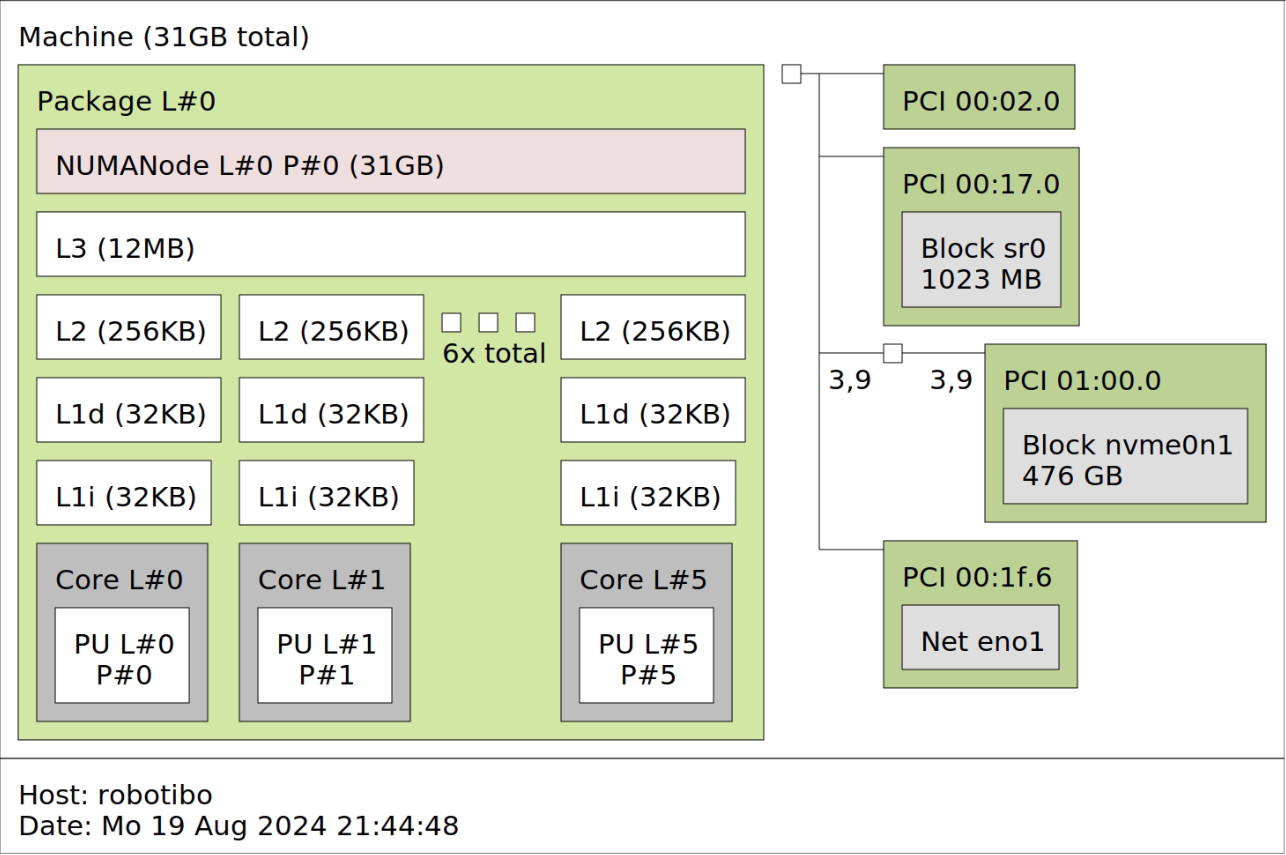
\includegraphics[width=1.0\columnwidth]{img/lstopo.png}
	\caption[Hardware topology]{Hardware topology}
	\label{fig:lstopo}
\end{figure}


\clearpage

\chapter{Salamander 4}\label{cha:salamander4}
This chapter briefly describes the Salamander 4 operating system by SIGMATEK. 

\section{Structure}
\noindent Salamander 4 is the proprietary operating system of SIGMATEK. It is based on Linux version 5.15.94 and integrates Xenomai 3.2, a real-time development environment~\cite{XenomaiXenomai}. Salamander 4 is a 64-bit system, which refers to the x86\_64 architecture. The real-time behaviour is achieved through the use of Symmetric Multi-Processing (SMP) and Preemptive Scheduling (PREEMPT). In addition, it uses IRQPIPE to process interrupts in a way that meets the real-time requirements of the system. The output of the command \texttt{uname -a} can be observed in code~\ref{output:uname_a_virt}.

\vspace{1em}
\begin{minipage}{0.95\columnwidth}
	\begin{lstlisting}[name={System information},label={output:uname_a_virt}]
root@sigmatek-core2:~# uname -a
Linux sigmatek-core2 5.15.94 #1 SMP PREEMPT IRQPIPE Tue Feb 14 18:18:05 UTC 2023 x86_64 GNU/Linux
\end{lstlisting}
\end{minipage}

\noindent Salamander 4 is powered by SIGMATEK's CP 841~\cite{CPUEinheitenSIGMATEK} and is comprised of the following software modules:

 \begin{itemize}
	\item \textbf{Operating system}: The operating system in a LASAL CPU manages the hardware and software resources of the system. It is provided in a completely PC-compatible manner, working with a standard PC BIOS.
	\item \textbf{Loader}: The loader is a part of the operating system that is responsible for loading programs from executables into memory, preparing them for execution and then executing them.
	\item \textbf{Hardware classes}: Hardware classes in LASAL represent the different types of hardware components that can be controlled by the LASAL CPU. They provide a way to organize and manage the hardware components in a modular and reusable manner. The graphical hardware editor in LASAL allows for a true-to-detail simulation of the actual hardware.
	\item \textbf{Application}: Applications are developed using LASAL CLASS 2~\cite{EngineeringToolLASAL}, a solution for automation tasks that supports object-oriented programming and design in compliance with IEC 61131-3.
\end{itemize}


\clearpage
\noindent The interfaces between the individual modules are indicated by an arrow in Figure~\ref{fig:lasal_cpu}.

\begin{figure}[H]
	\centering
	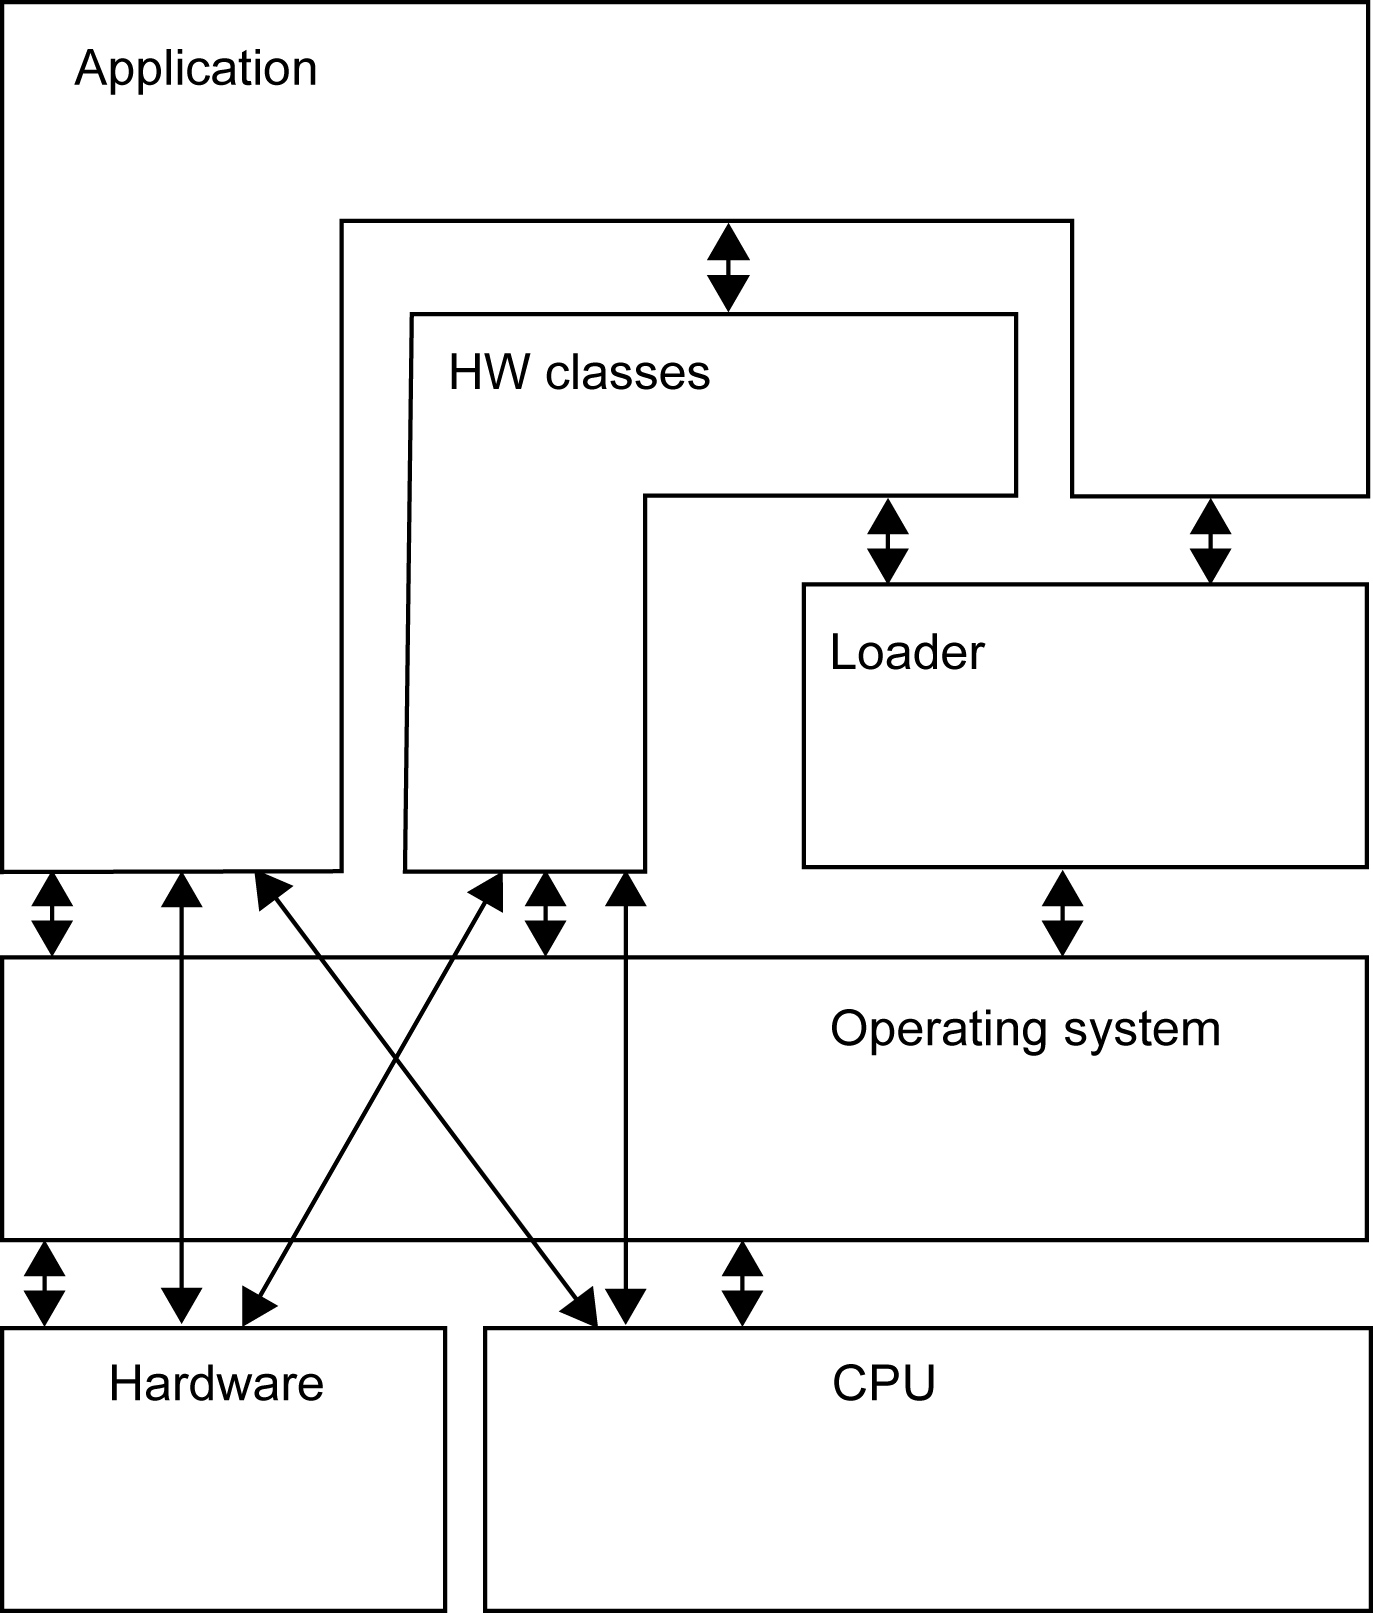
\includegraphics[width=0.5\columnwidth]{img/Software-Struktur_einer_LASAL_CPU.png}
	\caption[Structure of Salamander 4 CPU]{Structure of Salamander 4 CPU}
	\label{fig:lasal_cpu}
\end{figure}

\section{Memory Management}
\noindent For the sake of completeness, Figure~\ref{fig:memory_management} displays the memory management of Salamander 4. LRT stands for Lasal Runtime and creates an execution environment where applications developed using the LASAL Class 2 can run, providing defined real-time functions, data types, and other constructs tailored for real-time programming.

\begin{figure}[H]
	\centering
	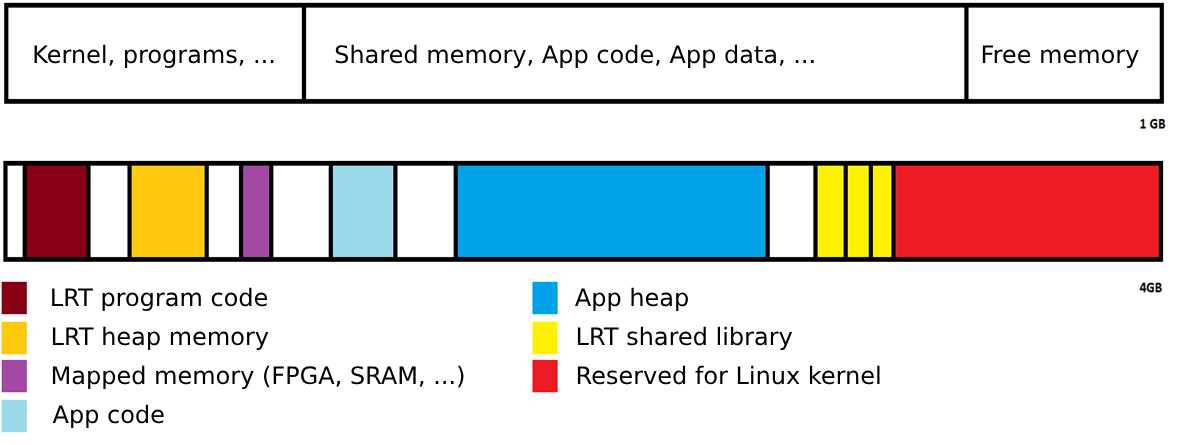
\includegraphics[width=0.8\columnwidth]{img/RAM_Memory_management.png}
	\caption[Memory Management]{Memory Management}
	\label{fig:memory_management}
\end{figure}

\clearpage

\section{Xenomai}
\noindent Xenomai 3~\cite{XenomaiXenomai} is a real-time framework that offers two paths to real-time performance. The first approach supplements the Linux kernel with a compact real-time core dubbed Cobalt, demonstrated in Figure~\ref{fig:cobalt}. Cobalt runs side-by-side with Linux, but it handles all time-critical activities like interrupt processing and real-time thread scheduling with higher priority than the regular kernel activities. 

\begin{figure}[H]
	\centering
	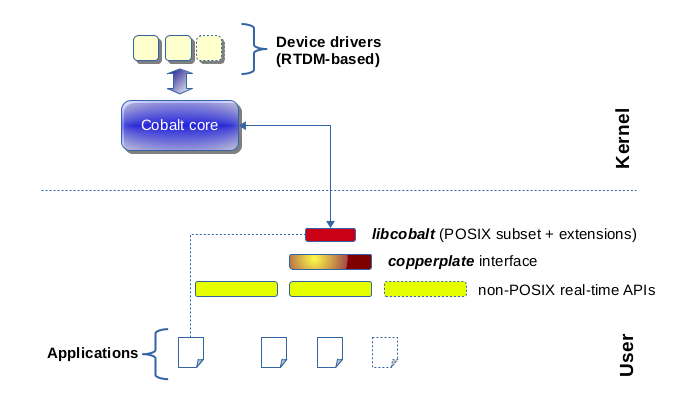
\includegraphics[width=0.6\columnwidth]{img/x3-cobalt-interfaces.png}
	\caption[Xenomai Cobalt interfaces]{Xenomai Cobalt interfaces}
	\label{fig:cobalt}
\end{figure}

\bigskip \noindent  The second approach, called Mercury and shown in Figure~\ref{fig:mercury}, relies on the real-time capabilities already present in the native Linux kernel. Often, applications require the PREEMPT-RT extension to augment the mainline kernel's real-time responsiveness and minimize jitter, but this isn't mandatory and depends on the application's specific requirements for responsiveness and tolerance for occasional deadline misses. 


\begin{figure}[H]
	\centering
	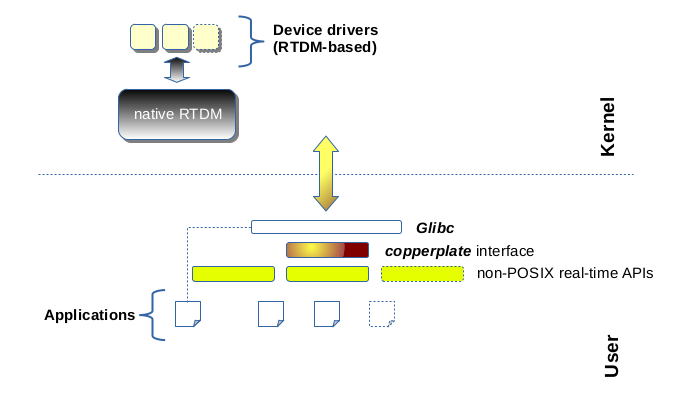
\includegraphics[width=0.6\columnwidth]{img/x3-mercury-interfaces.png}
	\caption[Xenomai Mercury interfaces]{Xenomai Mercury interfaces}
	\label{fig:mercury}
\end{figure}

\noindent Salamander 4 uses the Cobalt real-time core with the Dovetail extension, which allows the kernel to handle real-time tasks with low latency.

\clearpage

\chapter{Initial Real-Time Latency}\label{cha:initial-real-time-latency}

As a starting point, initial latency values of both the bare metal and virtualization versions were measured with the latency tool of the xenomai tool suite. Salamander 4 bare metal refers to the proprietary hardware of SIGMATEK used to employ the custom operating system. Salamander 4 virtualization refers to a virtual version of the Salamander 4 hardware platform, achieved through QEMU/KVM. Sections~\ref{sec:salamander4-bare-metal} and~\ref{sec:salamander4-virtualization} specify the details of the measurements for both versions. In the further course, the aim was to bring the latency values of the virtualization closer to those of the hardware and guarantee deterministic and reliable behavior. 

\section{Salamander 4 Bare Metal}\label{sec:salamander4-bare-metal}
The output of the command \texttt{uname -a} for Salamander 4 bare metal is shown in code~\ref{output:uname_a_hw}.

\vspace{1em}
\begin{minipage}{0.95\columnwidth}
	\begin{lstlisting}[name={Salamander 4 bare metal system information},label={output:uname_a_hw}]
root@sigmatek-core2:~# uname -a 
Linux sigmatek-core2 5.15.94 #1 SMP PREEMPT IRQPIPE Tue Feb 14 18:18:05 UTC 2023 x86_64 GNU/Linux
\end{lstlisting}
\end{minipage}

\noindent As a reference point, the latency program was executed on Salamander 4 bare metal for a duration of 10 minutes. The complete command used was \texttt{latency -h -g gnuplot.txt -T 600}, which runs the latency measurement tool for 600 seconds and prints histograms of min, avg, max latencies in a Gnuplot-compatible format to the file \texttt{gnuplot.txt}. Figure~\ref{fig:max_latency_hardware} shows the gathered latency values in microseconds.

\begin{figure}[H]
	\centering
	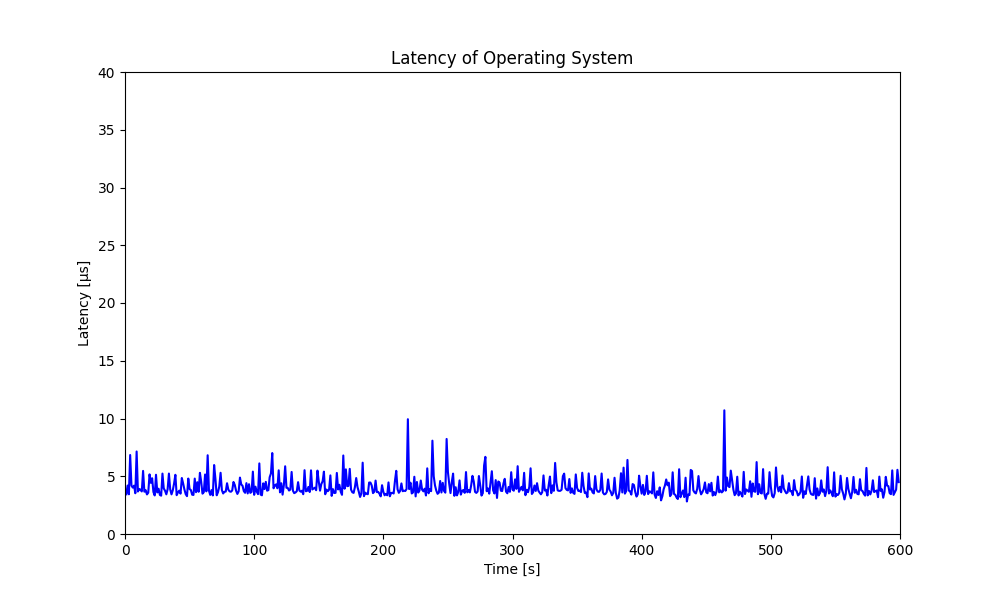
\includegraphics[width=1.0\columnwidth]{img/max_latency_hardware.png}
	\caption[Latency of Salamander 4 bare metal]{Latency of Salamander 4 bare metal}
	\label{fig:max_latency_hardware}
\end{figure}

\noindent The statistics obtained from this measurement are provided in Table~\ref{tab:latency_statistics_bare_metal}. It gives an overview of the average, maximum, minimum latency, and the standard deviation of the latency values in microseconds. 

\begin{table}[h]
	\centering
	\caption{Latency statistics of Salamander 4 bare metal in microseconds}
	\label{tab:latency_statistics_bare_metal}
	\begin{tabular}{|c|c|}\hline
	\textbf{Statistic} & \textbf{Value (\textmu s)} \\\hline
	Average Latency & 4.06 \\\hline
	Maximum Latency & 10.71 \\\hline
	Minimum Latency & 2.82 \\\hline
	Standard Deviation & 0.85 \\\hline
	\end{tabular}
	\end{table}

\noindent Figure~\ref{fig:gnuplot_max_latency_hardware} depicts the variation in latency over the course of said time. Since the data varies strongly, a logarithmic scale was used for both axes.

\begin{figure}[H]
	\centering
	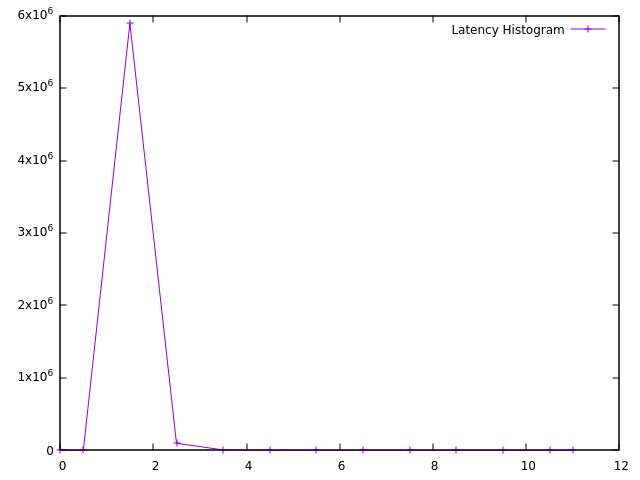
\includegraphics[width=0.7\columnwidth]{masterthesis-documentation/docs/sigmatek/xenomai/0hardware/gnuplot_max_latency_hardware.png}
	\caption[Variation in latency of Salamander 4 bare metal]{Variation in latency of Salamander 4 bare metal}
	\label{fig:gnuplot_max_latency_hardware}
\end{figure}


\section{Salamander 4 Virtualization}\label{sec:salamander4-virtualization}
In addition to providing Salamander 4 on its own hardware, SIGMATEK has also developed a virtualised version of this operating system. It was developed using Yocto, an open-source project that allows customised Linux distributions to be created for embedded systems~\cite{WelcomeYoctoProject}. Upon generating the necessary files, Yocto provides a QEMU folder with the following components shown in code~\ref{lst:ls}. QEMU is the environment in which the virtualization runs, as it is an open-source tool for hardware virtualization~\cite{QEMU}.

\vspace{1em}
\begin{minipage}{\linewidth}
	\begin{lstlisting}[name={Contents of QEMU folder for Salamander 4},label={lst:ls}]
    sigma_ibo@localhost:~/Desktop/salamander-image$ ls -1
    bzImage
    drive-c
    ovmf.code.qcow2
    qemu_def.sh
    salamander-image-sigmatek-core2.ext4
    stek-drive-c-image-sigmatek-core2.tar.gz
    vmlinux
    \end{lstlisting}
\end{minipage}

\noindent With the help of the script depicted in code~\ref{script:qemu_def}, Salamander 4 is started together with the necessary hardware components in the QEMU environment. This makes it possible to run Salamander 4 on a variety of host systems, regardless of the specific hardware of the host. The following is a description of the components used for the virtualization of Salamander 4:
\begin{itemize}
	\item \textbf{bzImage}: Compressed Linux kernel image that is loaded by QEMU at system start. ``bz`` stands for big-zipped.
	\item \textbf{drive-c}: Directory serving as C drive for QEMU system, created and filled by qemu\_def.sh script.
	\item \textbf{ovmf.code.qcow2}: Firmware file for QEMU that enables UEFI boot process. \texttt{OVMF} stands for Open Virtual Machine Firmware, \texttt{qcow2} is a format for disk image files used by QEMU, it stands for "QEMU Copy On Write version 2".
	\item \textbf{qemu\_def.sh}: Shell script that starts QEMU with required parameters to boot Salamamder 4 OS. It is described in Code~\ref{script:qemu_def}.
	\item \textbf{salamander-image-sigmatek-core2.ext4}: Disk image of the Salamander 4 OS for the Sigmatek Core 2 platform. It uses the \texttt{ext4} file system and serves as the root file system in the QEMU virtual machine, acting as the virtual hard drive.
	\item \textbf{stek-drive-c-image-sigmatek-core2.tar.gz}: Compressed tarball containing a pre-configured environment for the Salamander 4 OS. It is unpacked and sets up the \texttt{drive-c/} directory with system and log files in the \texttt{qemu\_def.sh} script. 
	\item \textbf{vmlinux}: Uncompressed Linux kernel image, typically used for debugging.
\end{itemize}


\begin{comment}
	https://www.baeldung.com/linux/kernel-images
\end{comment}


\noindent The inital QEMU script after the custom Yocto build and the starting point for this work is shown in Code~\ref{script:qemu_def}. This script is used to start QEMU with required parameters to boot Salamamder 4 OS. It will be adjusted in chapter~\ref{cha:real-time_tuning} in order to accompany real-time performance tunings. 

\vspace{1em}
\begin{minipage}{\linewidth}
	\begin{lstlisting}[name={QEMU script for starting Salamander 4 virtualization},label={script:qemu_def}]
	#!/bin/sh

	if  [ ! -d drive-c/ ]; then
			echo "Filling drive-c/"
			mkdir drive-c/
			tar -C drive-c/ -xf stek-drive-c-image-sigmatek-core2.tar.gz
	fi
		
	exec qemu-system-x86_64 -M pc,accel=kvm -kernel ./bzImage \
	-m 2048 -drive file=salamander-image-sigmatek-core2.ext4,format=raw,media=disk \
	-append "console=ttyS0 console=tty1 root=/dev/sda rw panic=1 sigmatek_lrt.QEMU=1 ip=dhcp rootfstype=ext4" \
	-net nic,model=e1000,netdev=e1000 -netdev bridge,id=e1000,br=nm-bridge \
	-fsdev local,security_model=none,id=fsdev0,path=drive-c -device virtio-9p-pci,id=fs0,fsdev=fsdev0,mount_tag=/mnt/drive-C \
	-device vhost-vsock-pci,guest-cid=3,id=vsock0 \
	-drive if=pflash,format=qcow2,file=ovmf.code.qcow2 \
	-no-reboot -nographic
\end{lstlisting}
\end{minipage}

\noindent This script is run on a generic Ubuntu 22.04.4 system, as mentioned previously in chapter~\ref{cha:methodology}. The kernel version and other details are presented in Code~\ref{output:uname_a_ub}, using the \texttt{uname -a} command.

\vspace{1em}
\begin{minipage}{0.95\columnwidth}
	\begin{lstlisting}[name={Ubuntu 22.04.4 system information},label={output:uname_a_ub}]
root@sigmatek-core2:~# uname -a 
Linux sigma-ibo 6.5.0-35-generic #35~22.04.1-Ubuntu SMP PREEMPT_DYNAMIC Tue May  7 09:00:52 UTC 2 x86_64 x86_64 x86_64 GNU/Linux
\end{lstlisting}
\end{minipage}

\noindent Measuring the latency of the Salamander 4 virtualization with the default QEMU script in Code~\ref{script:qemu_def} and no further adjustments for 10 minutes, the following latency values in Figure~\ref{fig:max_latency_default} were collected. 

\begin{figure}[H]
	\centering
	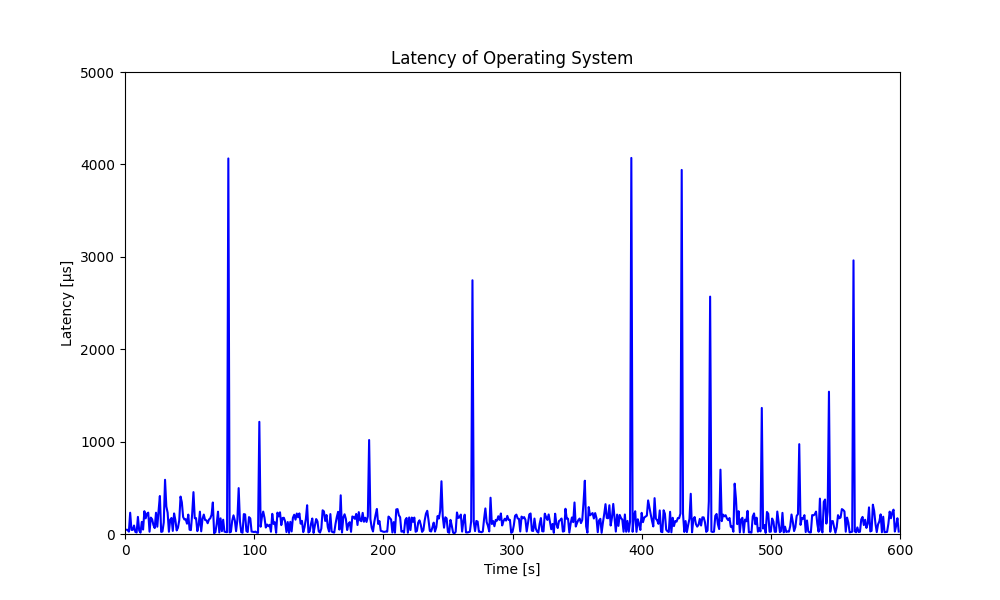
\includegraphics[width=0.75\columnwidth]{img/max_latency_default.png}
	\caption[Latency with default settings]{Latency with default settings}
	\label{fig:max_latency_default}
\end{figure}

\noindent The statistics obtained from this measurement are provided in Table~\ref{tab:latency_statistics_virt}. It gives an overview of the average, maximum, minimum latency, and the standard deviation of the latency values in microseconds. 

\begin{table}[h]
	\centering
	\caption{Latency statistics of default Salamander 4 virtualization in microseconds}
	\label{tab:latency_statistics_virt}
	\begin{tabular}{|c|c|}\hline
	\textbf{Statistic} & \textbf{Value (\textmu s)} \\\hline
	Average Latency & 46.22 \\\hline
	Maximum Latency & 707.62 \\\hline
	Minimum Latency & 15.59 \\\hline
	Standard Deviation & 52.13 \\\hline
	\end{tabular}
	\end{table}

\noindent Figure~\ref{fig:gnuplot_max_latency_default} depicts the variation in latency over the course of said time with default settings. 

\begin{figure}[H]
	\centering
	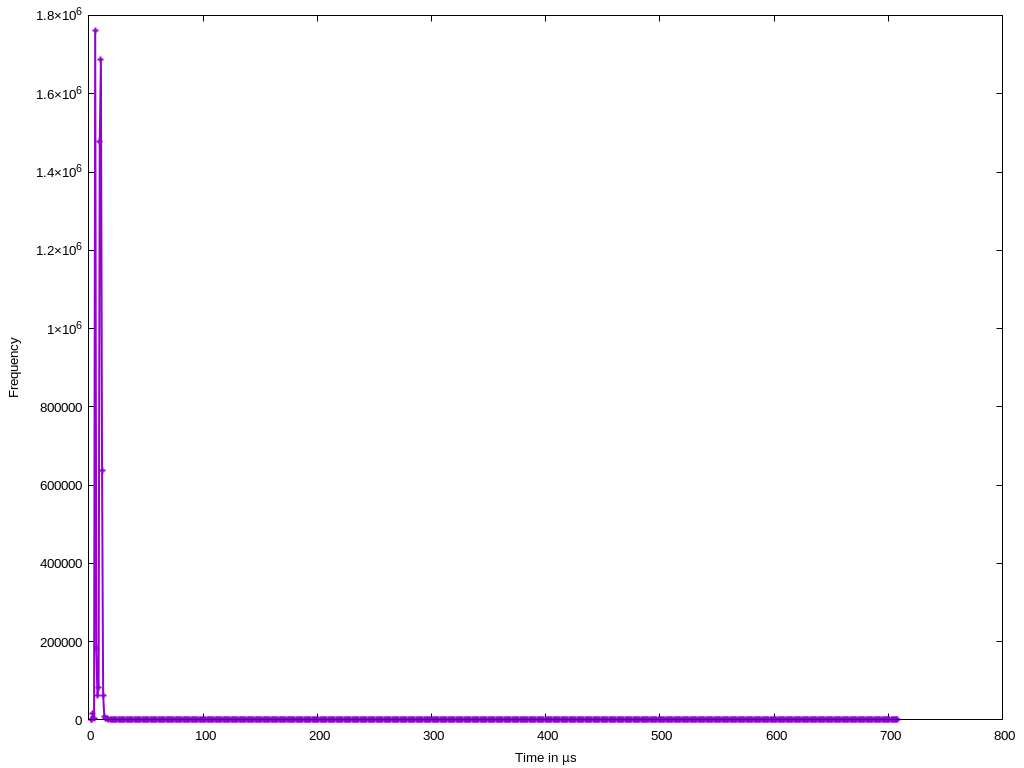
\includegraphics[width=0.7\columnwidth]{masterthesis-documentation/docs/sigmatek/xenomai/1default/gnuplot_max_latency_default.png}
	\caption[Variation in latency with default settings]{Variation in latency with default settings}
	\label{fig:gnuplot_max_latency_default}
\end{figure}


\noindent Comparing these values to those of bare metal in Figure \ref{fig:gnuplot_max_latency_combined}, it is evident that there is a significant initial gap in the statistics. A maximum latency of 707.62~\textmu s is not tolerable for the system and needs to be tuned. 

\begin{figure}[H]
	\centering
	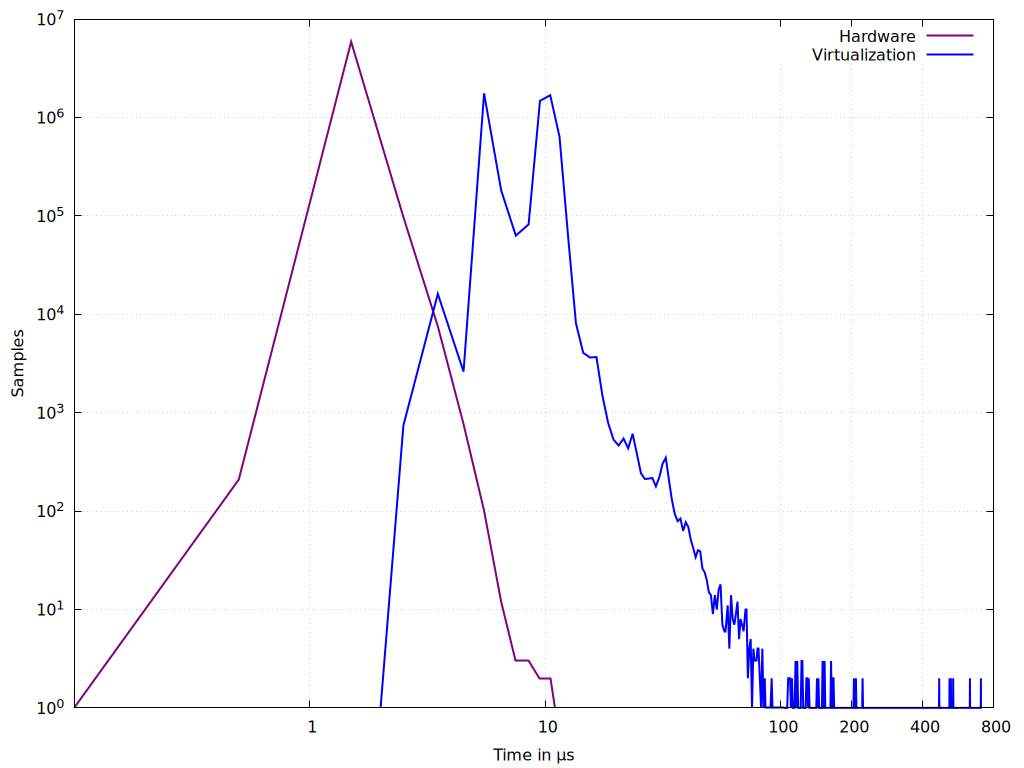
\includegraphics[width=0.7\columnwidth]{masterthesis-documentation/docs/sigmatek/xenomai/01combined/gnuplot_combined_max_latency.png}
	\caption[Comparison of variation in latency between hardware and virtualization]{Comparison of variation in latency between hardware and virtualization}
	\label{fig:gnuplot_max_latency_combined}
\end{figure}



\clearpage

\chapter{Real-Time Performance Tuning}\label{cha:real-time_tuning}

In this chapter, the significant initial gap in latency statistics between the virtualized system and the bare metal system is tackled. For this reason, an extensive tuning process is carried out. This involves configurations spanning the BIOS, kernel, host OS, QEMU-KVM virtualization layer, and the Salamander 4 OS itself. The individual configurations will be discussed in detail and the modifications will be justified with a clear explanation. The goal is to bring the latency of the virtualized system closer to that of the bare metal system, thereby ensuring deterministic behavior under real-time constraints.

\section{BIOS Configurations}

BIOS stands for Basic Input/Output System. It abstracts the hardware and enables basic functions of a computer during the booting process, such as starting the operating system and loading other software. Since the BIOS is embedded very deep, its configuration can significantly influence the real-time performance of the system. Table~\ref{tab:bios_configuration} illustrates the specific BIOS settings that have been adjusted for the purpose of real-time performance. 

\begin{table}[h]
	\centering
	\caption{BIOS Configurations}
	\label{tab:bios_configuration}
	\setlength{\tabcolsep}{0.5em} % for the horizontal padding
	{\renewcommand{\arraystretch}{1.2}% for the vertical padding
	\begin{tabular}{|l|l|}
	\hline
	\textbf{Option} & \textbf{Status} \\
	\hline
	Hyper Threading & Disabled \\
	\hline
	Intel SpeedStep® & Disabled \\
	\hline
	Intel® Speed Shift Technology & Disabled \\
	\hline
	C States & Disabled \\
	\hline
	VT-d & Enabled \\
	\hline
	\end{tabular}}
	\end{table}	
	
	\noindent In the following, these settings along with their impact on system latency are briefly described. 

	\begin{itemize}
		\item \textbf{Hyper Threading}: Hyper-Threading allows CPUs to process two threads simultaneously instead of just one. When it is enabled on the host, this allows the parallelisation of tasks and increases performance. However, in a real-time system like the guest Salamander 4, this can lead to increased latencies due to contention between threads. In order to ensure more deterministic behavior in the guest, it is disabled on the host.
		\item \textbf{Intel SpeedStep}: This technology dynamically adjusts the clock speed of the CPU based on workload. These dynamic changes can lead to unpredictable latencies in a real-time system. It is also disabled on the host to maintain a constant CPU speed.
		\item \textbf{Intel® Speed Shift Technology}: Similar to SpeedStep, Speed Shift allows the processor to directly control its frequency and voltage. This can lead to unpredictable latencies, too. Hence, it is also disabled on the host.
		\item \textbf{C States}: These are low-power idle states where the clock frequency and voltage of the CPU are reduced. Transitioning between C-states can cause variable latencies. To prevent this from happening, C-states are disabled on the host.
		\item \textbf{VT-d}: Direct access to physical devices from within virtual machines is possible when VT-d is enabled on the host. This can help reduce latencies associated with I/O operations in the virtual machine. It is therefore enabled on the host.
	\end{itemize}

\section{Kernel Configurations}

The kernel command-line parameters are shown in Code~\ref{script:kernel_cli} below. Some of them are essential for real-time performance.

\vspace{1em}
\begin{minipage}{0.95\columnwidth}
	\begin{lstlisting}[name={Kernel Configuration},label={script:kernel_cli}]
		GRUB_CMDLINE_LINUX="isolcpus=4 rcu_nocbs=4 nohz_full=4 nohz=on default_hugepagesz=1G hugepagesz=1G hugepages=8 intel_iommu=on rdt=l3cat nmi_watchdog=0 idle=poll clocksource=tsc tsc=reliable audit=0 skew_tick=1 intel_pstate=disable intel.max_cstate=0 intel_idle.max_cstate=0 processor.max_cstate=0 processor_idle.max_cstate=0 nosoftlockup no_timer_check nospectre_v2 spectre_v2_user=off kvm.kvmclock_periodic_sync=N kvm_intel.ple_gap=0 irqaffinity=0"
\end{lstlisting}
\end{minipage}

\noindent In the following, these settings along with their impact on system latency are briefly described. 

\begin{itemize}
	\item \textbf{isolcpus=4}: Isolates CPU 4 from the general scheduler, meaning no process will be scheduled to run on this CPU unless it is explicitly assigned. CPU isolation is explained in detail in section \ref{sec:cpu_isolation}.
	\item \textbf{rcu\_nocbs=4}: The Linux kernel uses a synchronization mechanism called RCU, or Read-Copy-Update. It lets writers update the data in a way that guarantees readers will always see the same version while enabling multiple readers to access shared data without locks. The RCU subsystem uses callback functions that need to be invoked once readers are done with the data they accessed. By default, these callbacks are handled by the CPUs that executed the read-side critical sections. This parameter offloads RCU callback handling from CPU 4 to other CPUs. CPU 4 remains dedicated to high-priority tasks which helps in reducing latency.
	\item \textbf{nohz\_full=4}: Makes CPU core 4 "tickless", meaning the kernel tries to avoid sending periodic scheduling-clock interrupts to the CPU when there are no runnable tasks. This lowers latency by reducing unnecessary wake-ups but may increase power consumption because the CPU is not able to enter a low-power state when idle. Additionally, timer interrupts cannot be fully eliminated because certain events, such as incoming interrupts or task activations, can still cause the kernel to send timer interrupts to the tickless CPU.	
	\item \textbf{nohz=on}: Sets all CPUs to tickless mode system-wide.
	\item \textbf{default\_hugepagesz=1G, hugepagesz=1G, hugepages=8}: Huge pages are large contiguous areas of memory that can be used by applications and the kernel, instead of the traditional 4KB small pages. The default huge page size is set to 1GB, and 8 huge pages of 1GB size are reserved at boot. This pre-allocation makes sure that these large memory regions are available to be used by the kernel or applications, without having to dynamically allocate and potentially fail.
	\item \textbf{intel\_iommu=on}: Enables Intel's IOMMU (Input/Output Memory Management Unit), which connects a DMA (Direct Memory Access)-capable I/O bus, such as graphics cards and network adapters, to the main memory. It can enhance device performance by allowing these devices to directly access and use memory, which is especially helpful when these devices are virtualized.
	\item \textbf{rdt=l3cat}: Activates the L3 CAT (L3 Cache Allocation Technology) feature of Intel’s RDT (Resource Director Technology). Unlike L1 and L2 caches, where each core has its fixed capacity, L3 cache is a shared pool among multiple cores. L3 CAT is a mechanism that controls the amount of L3 cache that a process can use. By controlling cache allocation, it can prevent a single process from monopolizing the L3 cache, which is particularly beneficial in virtualized environments, where multiple virtual machines share the same physical host.
	\item \textbf{nmi\_watchdog=0}: Disables the NMI (Non-Maskable Interrupt) watchdog, which is a debugging feature of the Linux kernel. It works by periodically generating non-maskable interrupts. If the system does not respond to these interrupts within a certain timeframe, the NMI watchdog concludes that the system has hung and generates a system dump for debugging.  This constant monitoring consumes CPU cycles and can introduce undesirable latency in real-time systems.
	\item \textbf{idle=poll}: Changes the CPU’s idle loop behavior to active polling. Instead of entering a low-power state when idle, the CPU continuously polls for new tasks. This can reduce task start latency in real-time systems, but it increases power consumption.
	\item \textbf{clocksource=tsc, tsc=reliable}: TSC (Time Stamp Counter) is a high-resolution timer provided by most x86 processors that counts the number of CPU cycles since it was last reset. Accurate timekeeping is crucial, particularly for real-time systems. These parameters set the clocksource to TSC and mark it as a reliable source of timekeeping, meaning it increments at a consistent rate and does not stop when the processor is idle. 
	\item \textbf{audit=0}: Disables the Linux audit system. When it is enabled, it generates log entries for security-relevant events, which is a slow operation since they are written to disk. If there are a large number of such events, the audit system can consume significant CPU time and I/O bandwidth which could lead to higher latency.
	\item \textbf{skew\_tick=1}: Enables a mode in the Linux kernel that reduces timer interrupt overhead. Normally, timer interrupts happen simultaneously on all CPUs, resulting in all CPUs to exit their low-power states at once. This can lead to increased contention for system resources. When enabled, the kernel offsets the timer interrupts on different CPUs, spreading them out over time.
	\item \textbf{intel\_pstate=disable}: Disables the Intel P-state driver, which is a part of the Linux kernel that handles power management for Intel CPUs. It controls the frequency of the CPU by scaling it up when demand is high and scaling it down to save power when demand is low. This dynamic frequency scaling is disabled because it leads to increased latencies for real-time systems.
	\item \textbf{intel.max\_cstate=0, intel\_idle.max\_cstate=0, processor.max\_cstate=0, processor\_idle.max\_cstate=0}: These parameters disable deeper C-states (CPU power saving states). Normally, when a CPU is idle, it can enter various C-states, with higher-numbered states representing deeper sleep states that save more power but take longer to wake up from. In real-time systems, these wake-up delays can be problematic. Disabling them leads keeps the CPUs ready to respond quickly to new tasks and helps in reducing latency.
	\item \textbf{nosoftlockup}: Disables the soft lockup detector in the Linux kernel. A soft lockup is when a CPU is busy executing kernel code for a long period of time without giving other tasks a chance to run. Especially threads with SCHED\_FIFO policy occupy the CPU for an extensive duration. This is detected and reported by the soft lockup detector, hence it is disabled to prevent these unnecessary warnings.
	\item \textbf{no\_timer\_check}: Disables the check for broken timer interrupt sources. Broken timer interrupt sources are problems with hardware or software that prevent timer interrupts from working as intended. Such a timer may not generate interrupts at the expected rate or at all. The kernel skips the checks for these broken timer interrupt sources, which can cause unnecessary overhead in a real-time system where every CPU cycle counts.
	\item \textbf{nospectre\_v2, spectre\_v2\_user=off}: These parameters disable mitigations for the Spectre v2 vulnerability. Spectre v2 is a hardware vulnerability that affects many modern microprocessors and can allow malicious programs to access sensitive data they are not supposed to. While this is necessary for security, it has an impact on performance and should be turned off in controlled environments where the risk of exploitation is low.
	\item \textbf{kvm.kvmclock\_periodic\_sync=N, kvm\_intel.ple\_gap=0}: These are KVM (Kernel-based Virtual Machine) related parameters. They disable the periodic synchronization of the kvmclock and set the gap between PLE (Pause Loop Exiting) events to 0. The kvmclock is a paravirtualized clock source provided by KVM to its guest OS and disabling this reduces latency introduced by clock synchronization. By setting the gap to 0, the virtual machine exits the pause loop immediately, which can reduce latency in spinlock-intensive workloads.
	\item \textbf{irqaffinity=0}: Sets the default Interrupt Request affinity to none. This means that no CPU core is preferred over another for handling IRQs. Instead, it lets the operating system decide how to distribute these IRQs across all the CPUs. Section \ref{sec:irq_handling} dives deeper into Interrupt Request affinity.
\end{itemize}

\section{Host OS Configurations}
\subsection{CPU isolation}\label{sec:cpu_isolation}

Isolating CPUs involves removing all user-space threads and unbound kernel threads since bound kernel threads are tied to specific CPUs and hence cannot be moved. Also, modifying the \texttt{proc/irq/IRQ\_NUMBER/smp\_affinity} property of each Interrupt IRQ\_NUMBER in the system is part of this process, as described later in section~\ref{sec:irq_handling}. 

\noindent For CPU isolation, the \texttt{isolcpus} function was used to isolate a performance CPU from the general scheduling algorithms of the operating system. This means that the isolated CPUs will not be used for regular task scheduling, allowing them to be dedicated for the real-time specific tasks or processes. However, the isolcpus function only isolates at the user level and does not affect kernel tasks. Consequently, these kernel tasks and interrupts can still utilize the CPU~\cite{maPerformanceTuningKVMbased}. Output~\ref{output:pse} shows the user and kernel tasks that run on CPU 4. After the isolation, user tasks other than the QEMU process have been removed from running on this CPU. Only few critical kernel threads that are tied to this CPU still take CPU time.

\vspace{1em}
\begin{minipage}{0.95\columnwidth}
	\begin{lstlisting}[name={User and Kernel Tasks},label={output:pse},escapeinside={(*@}{@*)}]
		sigma_ibo@sigma-ibo:~$ cat /sys/devices/system/cpu/isolated
		4
		sigma_ibo@sigma-ibo:~$ ps axHo psr,pid,lwp,args,policy,nice,rtprio | awk '$1 == 4'
		4      38      38 [cpuhp/4]                   TS    0      -
		4      39      39 [idle_inject/4]             FF    -     50
		4      40      40 [migration/4]               FF    -     99
		4      41      41 [ksoftirqd/4]               TS    0      -
		4      43      43 [kworker/4:0H-events_highpr TS  -20      -
		4     505     505 [irq/189-iwlwifi:queue_1]   FF    -     50
		4     519     519 [irq/203-iwlwifi:exception] FF    -     50
		4    3008    3008 [kworker/4:1H-kblockd]      TS  -20      -
		4  177779  177779 [kworker/4:2-events]        TS    0      -
		4  448807  448807 [kworker/4:1-events]        TS    0      -		
\end{lstlisting}
\end{minipage}
\subsection{Interrupt Requests Handling}\label{sec:irq_handling}
Once the CPUs were isolated, Interrupt Requests handling was the next step. Interrupt Requests are used to send a signal to the CPU, prompting it to `interrupt' its current task and divert its attention to another task. This allows hardware devices to communicate with the CPU through frequent context switches, which can lead to performance degradation, especially in high-performance computing or real-time scenarios. To mitigate this, the IRQs needed to be removed from the isolated CPU. This was done by manipulating a file in the \texttt{proc} filesystem, namely \texttt{/proc/irq/<IRQ>/smp\_affinity}. The value in the \texttt{smp\_affinity} file is a bitmask in hexadecimal format. Each bit in this mask corresponds to a CPU in the system. The least significant bit (LSB) on the right corresponds to the first CPU (CPU0), and the significance increases towards the left until CPU19. In a system with 14 CPUs, if every CPU was reserved for one IRQ, the value for \texttt{smp\_affinity} would be 3FFF. The script in code~\ref{script:smp_affinity} was written to check and log the distribution of Interrupt Requests across each CPU in Salamander 4. 

\vspace{1em}
\begin{minipage}{0.95\columnwidth}
	\begin{lstlisting}[name={Check distribution of Interrupt Requests across each CPU},label={script:smp_affinity}]
		#!/bin/bash
		# Check if a command-line argument is provided
		if [ -z "$1" ]; then
			echo "Please provide a CPU number as a command-line argument."
			exit 1
		fi
		# Get the CPU number from the command-line argument
		CPU=$1
		# Initialize an empty array to store the IRQ numbers
		IRQs=()
		for IRQ in /proc/irq/*; do
			if [ -f "$IRQ/smp_affinity" ]; then
				# Read the current smp_affinity
				AFFINITY=$(cat "$IRQ/smp_affinity")
				# Check if the bit for the current CPU is set
				if (( (0x$AFFINITY & (1 << CPU)) != 0 )); then
					# Add the IRQ number to the array
					IRQs+=("${IRQ#/proc/irq/}")
				fi
			fi
		done
		# Sort the array
		IFS=$'\n' sorted=($(sort -n <<<"${IRQs[*]}"))
		# Print the CPU number
		echo "CPU $CPU IRQ affinity:"
		# Print the sorted IRQ numbers on separate lines
		for irq in "${sorted[@]}"; do
			echo "$irq"
		done
		
\end{lstlisting}
\end{minipage}


\noindent By changing the values of the \texttt{smp\_affinity} files of the respective IRQs, the assignment of IRQs was controlled so that they would not be handled by the isolated CPU. This reduced the interruptions caused by IRQs and the isolated CPUs were able to focus more on their assigned tasks.
\subsection{Disable dynamic frequency scaling}
\subsection{Disable RT throttling}
\subsection{No unexpected RT processes are running on your system}
\subsection{IRQ affinity}
\subsection{RCU CPU offloading}
\subsection{Suppress rcu cpu stall}
\subsection{Maybe?}
\subsection{Start QEMU normally and give all QEMU threads rt-priority} 
\subsection{Kill all running user processes}
\subsection{Set CPU Affinity for systemd services}
\subsection{Cache Isolation for CPU and GPU}
\subsection{Set CPU Affinity of IRQ thread to CPU 0}
\subsection{Set Device Driver Work Queue to CPU 0}
\subsection{Disable Machine Check}
\subsection{Stop Certain Services}
\section{QEMU-KVM Configurations}
\subsection{Tune lapic timer advance}
\subsection{Set QEMU options for real-time VM}
\subsection{Set CPU affinity and scheduling policy of QEMU CPU threads}
\subsection{Passthrough PCI devices into the VM}

\clearpage
\section{Guest OS Configurations}

\clearpage

\chapter{KVM exit reasons}\label{cha:kvm_exit_reasons}

\section{APIC\_WRITE}
\section{HLT}
\section{EPT\_MISCONFIG}
\section{PREEMPTION\_TIMER}
\section{EXTERNAL\_INTERRUPT}
\section{IO\_INSTRUCTION}
\section{EOI\_INDUCED}
\section{EPT\_VIOLATION}
\section{PAUSE\_INSTRUCTION}
\section{CPUID}
\section{MSR\_READ}

\clearpage

\chapter{Real-Time Robotic Application}\label{cha:real-time-testing}

\section{VARAN}
\section{Robotic Application}
\clearpage

\begin{comment}

\chapter{To Include}\label{cha:to_include}
\section{Latency Comparison}
In the initial phase, a comparative latency analysis was conducted between the hardware version and the virtualized version of Salamander 4. For this purpose, the latency tool of the Xenomai test suite was used. The latency was measured under two conditions, idle and CPU-stressed. The goal was to optimize the latency of the virtualization of Salamander 4 OS to closely match that of the bare metal version.

Vorgehensweise von~\cite{linPerformanceEvaluationXenomai}
\section{else}
Figure~\ref{fig:max_latency_vapic} shows latency of QEMU vapic Salamander4.
\begin{figure}[H]
	\centering
	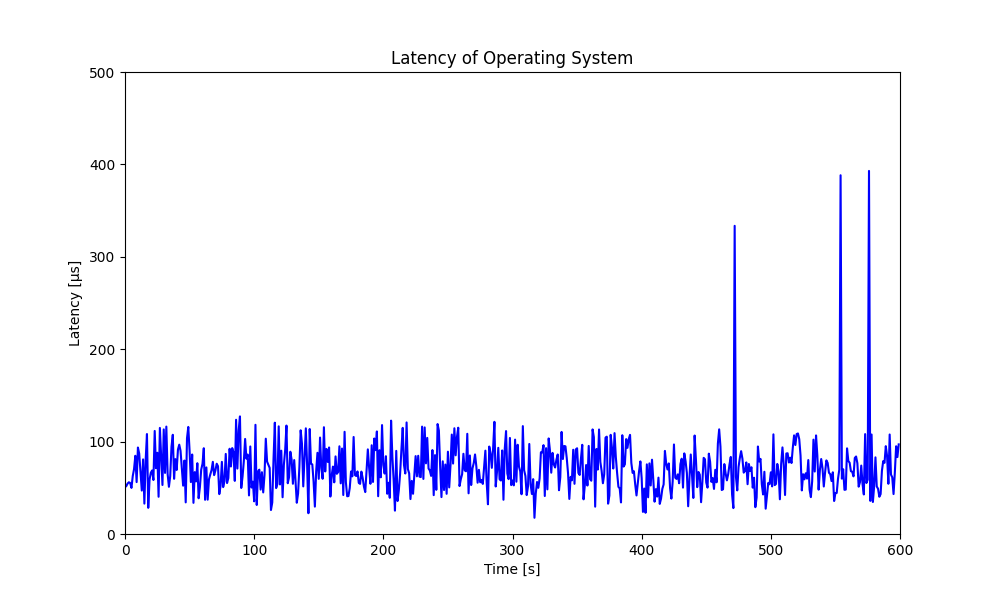
\includegraphics[width=0.75\columnwidth]{img/max_latency_vapic.png}
	\caption[Latency vapic]{Latency vapic}
	\label{fig:max_latency_vapic}
\end{figure}

After analyzing the inital latency of both versions, Trace-cmd and Kernelshark were used to further inspect the reasons that caused this divergence.

\noindent When the script is started from the host, the QEMU process can be scheduled to run on any available core, as it is not bound to a specific CPU core. This means that the QEMU process may frequently switch between different cores, leading to an increase in latency. As the goal was to reduce latency in the guest, the first step was to isolate a CPU of the host and dedicate it solely to the QEMU process, so that it cannot be used for other tasks on user level.


Figure~\ref{fig:max_latency_taskset} shows latency of QEMU taskset Salamander4.
\begin{figure}[H]
	\centering
	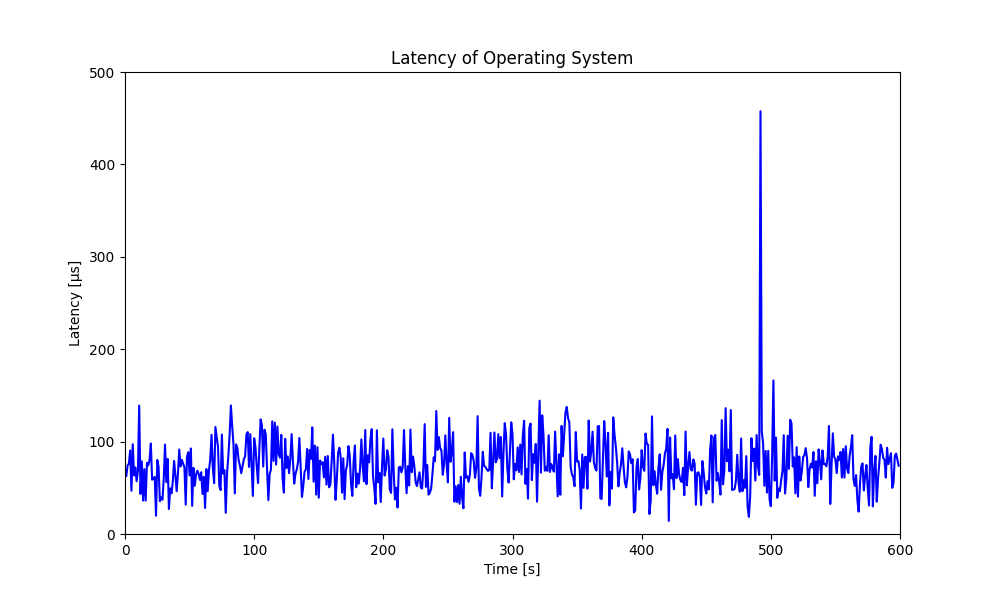
\includegraphics[width=0.75\columnwidth]{img/max_latency_taskset.png}
	\caption[Latency taskset]{Latency taskset}
	\label{fig:max_latency_taskset}
\end{figure}

\noindent Upon isolating a CPU to the QEMU process, it was anticipated that the guest would utilize nearly 100\% of the CPU's capacity, with minimal to no intervention from the host. However, the isolcpus function only isolates at the user level and does not affect kernel tasks. Consequently, these kernel tasks and interrupts can still utilize the CPU. This led to the investigation of the causes for the observed high and inconsistent latency. The guest operates within the kvm\_entry and \texttt{kvm\_exit} events of the host. Kernelshark revealed a high frequency of \texttt{kvm\_exit} events, indicating that the guest frequently relinquishes control of the CPU back to the host. This frequent switching hinders the guest\'s ability to run continuously, thereby increasing the virtualization latency. To further understand this, trace-cmd was employed to trace various events in the host-guest communication, including the reasons for these events. Specifically, the causes for \texttt{kvm\_exit} events were analyzed. The command sudo trace-cmd record -e all -A @3:823 --name Salamander4 -e all was executed on the host for a duration of 5 seconds. The results in Figure~\ref{fig:kvm_exit_taskset} were obtained. Additionally, Table~\ref{tab:kvm_exit} provides a short description of the observed \texttt{kvm\_exit} events.

\begin{table}[H]
	\centering
	\begin{tabular}{|l|p{0.62\textwidth}|}
		\hline
		\textbf{Exit Reason} & \textbf{Description}                                     \\
		\hline
		APIC\_WRITE          & Triggered when the guest writes to its APIC.             \\ \hline
		EXTERNAL\_INTERRUPT  & Triggered by external hardware interrupts.               \\ \hline
		HLT                  & Triggered when the guest executes the HLT instruction.   \\ \hline
		EPT\_MISCONFIG       & Triggered by a misconfiguration in the EPT.              \\ \hline
		PREEMPTION\_TIMER    & Triggered when the host's preemption timer expires.      \\ \hline
		PAUSE\_INSTRUCTION   & Triggered when the PAUSE instruction is executed.        \\ \hline
		EPT\_VIOLATION       & Triggered by a violation of the EPT permission settings. \\ \hline
		IO\_INSTRUCTION      & Triggered when the guest executes an I/O instruction.    \\ \hline
		EOI\_INDUCED         & Triggered when an EOI signal is sent to the APIC.        \\ \hline
		MSR\_READ            & Triggered when the guest reads from a MSR.               \\ \hline
		CPUID                & Triggered when the guest executes the CPUID instruction. \\ \hline
	\end{tabular}
	\caption{Description of kvm\_exit reasons}
	\label{tab:kvm_exit}
\end{table}

\clearpage
Figure~\ref{fig:kvm_exit_taskset} shows \texttt{kvm\_exit} frequency with CPU islation.
\begin{figure}[H]
	\centering
	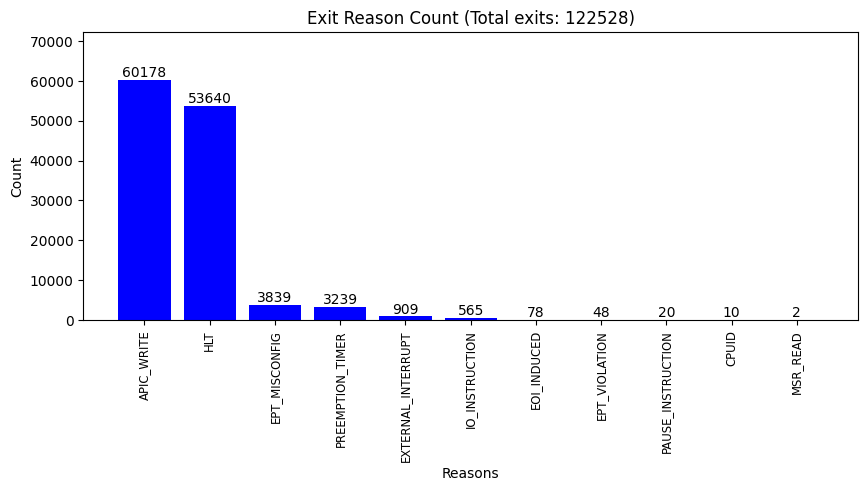
\includegraphics[width=1.0\columnwidth]{img/kvm_exits_taskset.png}
	\caption[kvm exits]{kvm exits}
	\label{fig:kvm_exit_taskset}
\end{figure}

Figure~\ref{fig:kvm_exits_default} shows \texttt{kvm\_exit} frequency without CPU islation.
\begin{figure}[H]
	\centering
	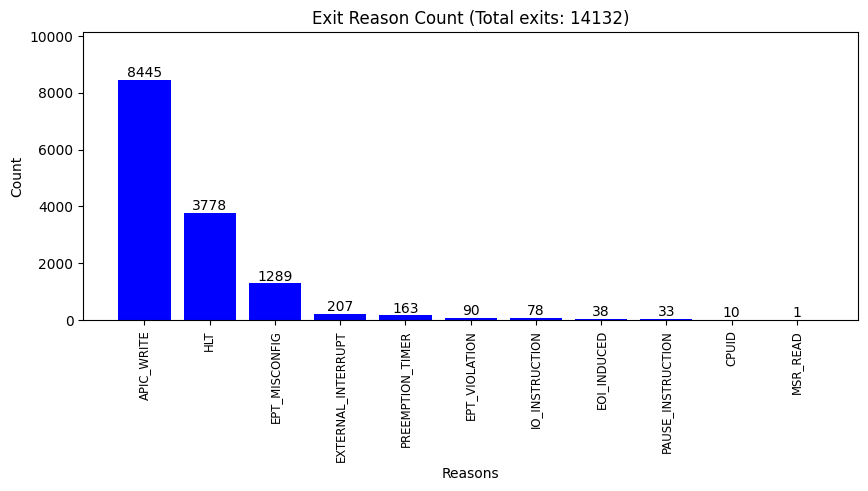
\includegraphics[width=1.0\columnwidth]{img/kvm_exits_default.png}
	\caption[kvm exits default]{kvm exits default}
	\label{fig:kvm_exits_default}
\end{figure}

\clearpage


\begin{table}[h!]
	\centering
	\begin{minipage}{.5\textwidth}
	\centering
	\caption{Host report CPU19 (Total of 445.908)}
	\label{tab:results_host_report}
	\begin{tabular}{|c|c|c|}
	\hline
	PID & Task & Count \\ \hline
	182579 & qemu-system-x86 & 302.748 \\ \hline
	0 & \textless{}idle\textgreater{} & 112.911 \\ \hline
	182618 & vhost & 21.204 \\ \hline
	182572 & qemu-system-x86 & 7.597 \\ \hline
	182755 & qemu-system-x86 & 644 \\ \hline
	182754 & qemu-system-x86 & 643 \\ \hline
	181870 & kworker/19:1 & 139 \\ \hline
	3820 & kworker/19:1H & 16 \\ \hline
	94 & migration/19 & 6 \\ \hline
	\end{tabular}
	\end{minipage}%
	\begin{minipage}{.5\textwidth}
	\centering
	\caption{Guest report (Total of 362.370)}
	\label{tab:results_guest_report}
	\begin{tabular}{|c|c|c|}
	\hline
	PID & Task & Count \\ \hline
	0 & \textless{}idle\textgreater{} & 150.744 \\ \hline
	331 & LRT-Main & 56.697 \\ \hline
	377 & trace-cmd & 48.507 \\ \hline
	346 & CLI & 26.426 \\ \hline
	378 & kthreadd & 25.837 \\ \hline
	340 & MainTaskLow & 19.291 \\ \hline
	339 & \textless{}...\textgreater{} & 9.980 \\ \hline
	34 & MainTaskHigh & 9.185 \\ \hline
	327 & LE-Logger & 4.965 \\ \hline
	369 & kworker/0:0 & 2.793 \\ \hline
	321 & kWorker-LRT & 2.542 \\ \hline
	328 & LRTMgr-Main & 1.651 \\ \hline
	34 & LrtMgrCyclic & 1.220 \\ \hline
	332 & cobalt\_printf & 1.112 \\ \hline
	325 & LE-System & 534 \\ \hline
	343 & TCP-Listen & 187 \\ \hline
	15 & rcu\_preempt & 162 \\ \hline
	25 & kcompactd0 & 122 \\ \hline
	58 & kworker/0:1H & 96 \\ \hline
	63 & kworker/u2:2 & 89 \\ \hline
	8 & jbd2/sda-8 & 86 \\ \hline
	22 & kworker/0:1 & 56 \\ \hline
	1 & init & 31 \\ \hline
	2 & kthreadd & 25 \\ \hline
	375 & trace-cmd & 24 \\ \hline
	14 & ksoftirqd/0 & 8 \\ \hline
	\end{tabular}
	\end{minipage}
	\end{table}

\noindent In the following, the host and guest tasks along with their impact on system latency are briefly described. 

\begin{itemize} 
	\item \textbf{qemu-system-x86}: Part of the QEMU process and specifically, this task emulates x86 systems. In Table~\ref{tab:results_host_report}, it occurs four times under different PIDs, hence there are four threads of it.
	\item \textbf{<idle>}: This represents the idle time of the CPU, hence it is not being used by any process, allowing to save power. The system halts until the next interrupt, which could be a timer interrupt, I/O interrupt, etc.
	\item \textbf{vhost}: A kernel module which improves virtual input/output (virtio) performance by handling virtqueues in the kernel, thereby reducing context switches and system calls. 
	\item \textbf{kworker/19:1}: A kernel worker thread created by the Linux kernel, kworker/19:1 performs work in response to system events. The number after the slash and colon indicate the CPU core and internal ID of the worker thread, respectively. 
	\item \textbf{kworker/19:1H}: Similar to kworker/19:1, kworker/19:1H is a kernel worker thread, with the ‘H’ suggesting that this thread handles hardware interrupts. 
	\item \textbf{migration/19}: The migration process is a kernel process that balances load across CPU cores by moving threads from one CPU to another. The number after the slash indicates the CPU core to which the migration process is bound. (URL: \url{https://elixir.bootlin.com/linux/latest/source/kernel/sched/core.c#L2325})

\end{itemize}

The Figure~\ref{fig:latency_comparison} below compares non-optimized guest latency with optimized guest latency and includes optimized bare-metal latency as a reference. The data shows that a 40\% reduction in QD1 latency is achievable through system tuning.

\begin{figure}[H]
	\centering
	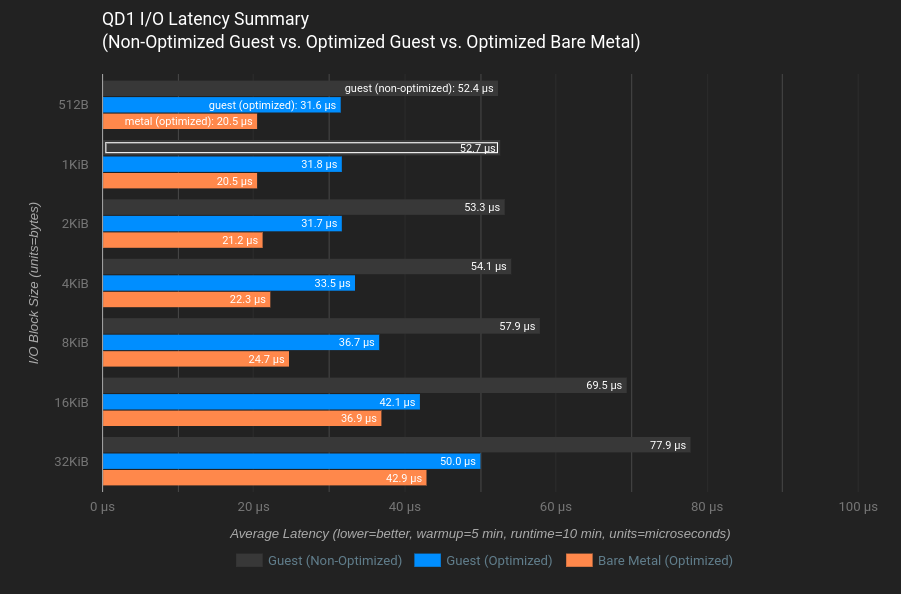
\includegraphics[width=1.0\columnwidth]{img/latency_comparison.png}
	\caption[latency comparison]{latency comparison}
	\label{fig:latency_comparison}
\end{figure}
\clearpage


\begin{table}[h]
	\centering
	\begin{tabular}{|p{0.1\textwidth}|p{0.45\textwidth}|p{0.45\textwidth}|}
	\hline
	\textbf{Number} & \textbf{Book} & \textbf{Citation} \\
	\hline
	\cite{maPerformanceTuningKVMbased} & Performance Tuning Towards a KVM-based Embedded Real-Time Virtualization System & It means that all threads, except for some per-core kernel threads, were prevented from running on the second processor core. \\
	\hline
	\cite{maPerformanceTuningKVMbased} & Performance Tuning Towards a KVM-based Embedded Real-Time Virtualization System & It means that all threads, except for some per-core kernel threads, were prevented from running on the second processor core. \\
	\hline
	\cite{maPerformanceTuningKVMbased} & Performance Tuning Towards a KVM-based Embedded Real-Time Virtualization System & It means that all threads, except for some per-core kernel threads, were prevented from running on the second processor core. \\
	\hline
	\cite{maPerformanceTuningKVMbased} & Performance Tuning Towards a KVM-based Embedded Real-Time Virtualization System & It means that all threads, except for some per-core kernel threads, were prevented from running on the second processor core. \\
	\hline
	\end{tabular}
	\caption{Your Caption}
	\label{tab:my_label}
	\end{table}
	
	Figure~\ref{fig:power_saver_kvm_exit} shows ...

	\begin{figure}[H]
		\centering
		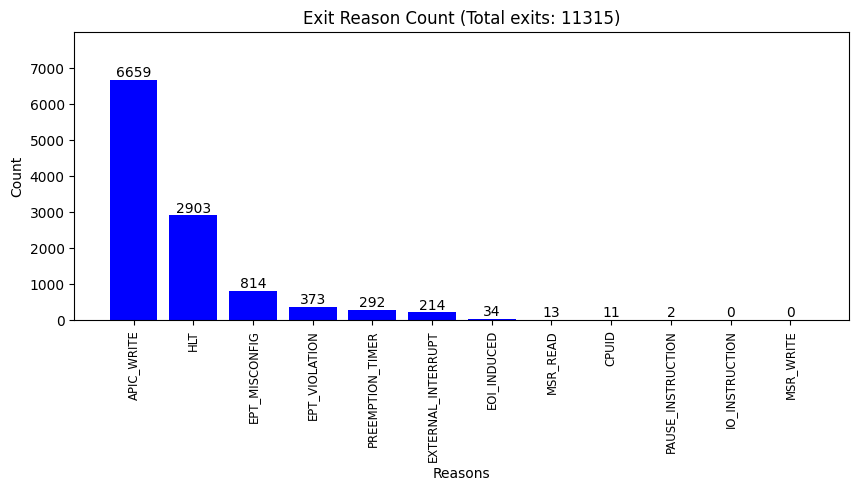
\includegraphics[width=1.0\columnwidth]{img/power_saver/kvm_exit_count.png}
		\caption[power\_saver kvm\_exit\_count]{power\_saver kvm\_exit\_count}
		\label{fig:power_saver_kvm_exit}
	\end{figure}
	\clearpage
	
	Figure~\ref{fig:power_saver_kvm_host} shows ...
	
	\begin{figure}[H]
		\centering
		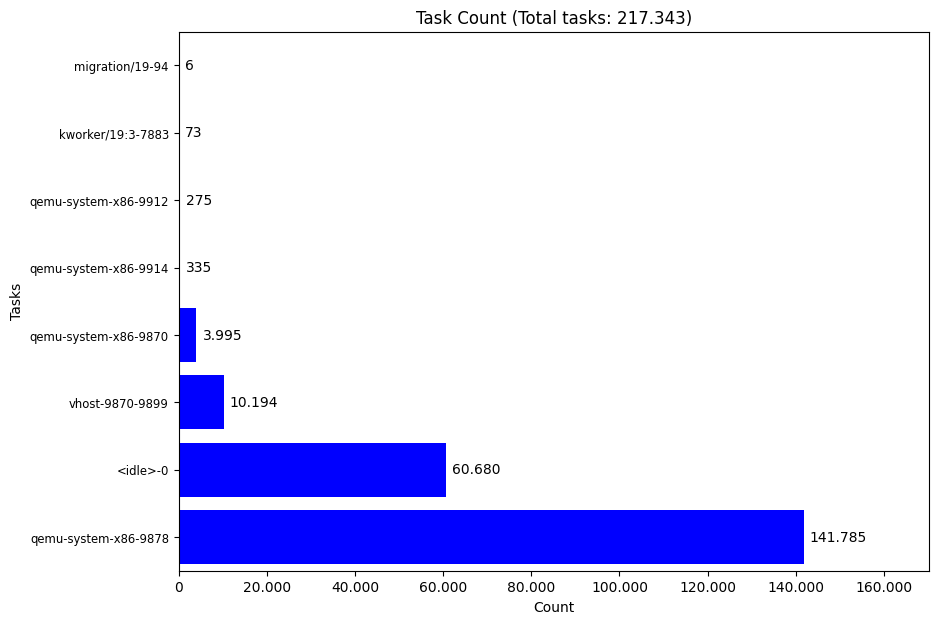
\includegraphics[width=1.0\columnwidth]{img/power_saver/results_host_report.png}
		\caption[power\_saver host report]{power\_saver host report}
		\label{fig:power_saver_kvm_host}
	\end{figure}
	\clearpage
	
	Figure~\ref{fig:power_saver_kvm_guest} shows ...
	
	\begin{figure}[H]
		\centering
		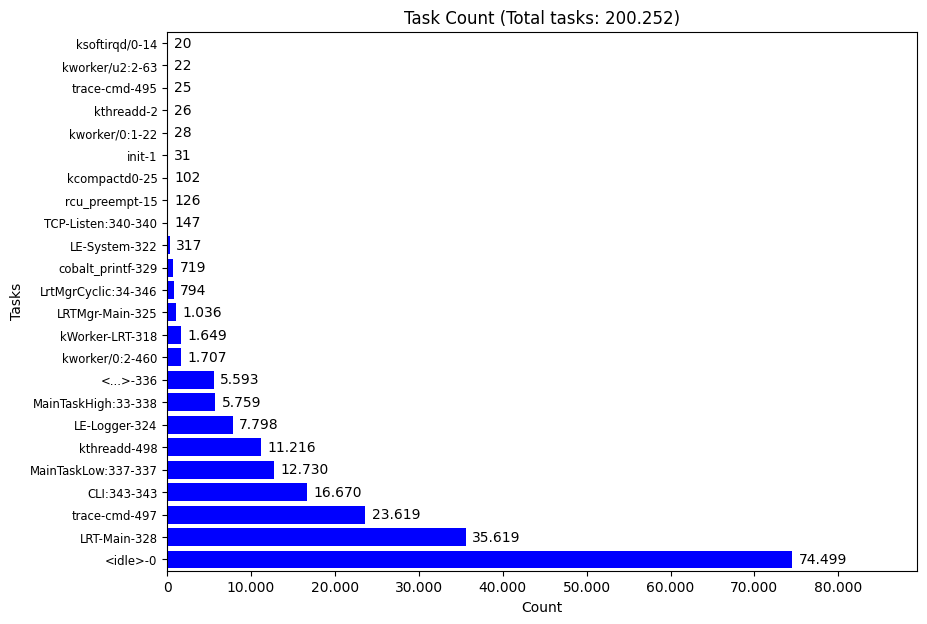
\includegraphics[width=1.0\columnwidth]{img/power_saver/results_guest_report.png}
		\caption[power\_saver guest report]{power\_saver guest report}
		\label{fig:power_saver_kvm_guest}
	\end{figure}
	\clearpage
	
	Figure~\ref{fig:balanced_kvm_exit} shows ...
	
	\begin{figure}[H]
		\centering
		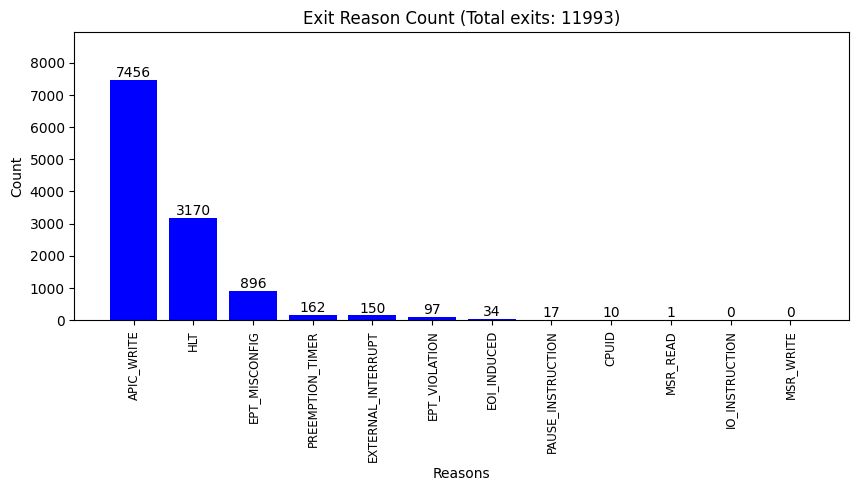
\includegraphics[width=1.0\columnwidth]{img/balanced/kvm_exit_count.png}
		\caption[balanced kvm\_exit\_count]{balanced kvm\_exit\_count}
		\label{fig:balanced_kvm_exit}
	\end{figure}
	\clearpage
	
	Figure~\ref{fig:balanced_kvm_host} shows ...
	
	\begin{figure}[H]
		\centering
		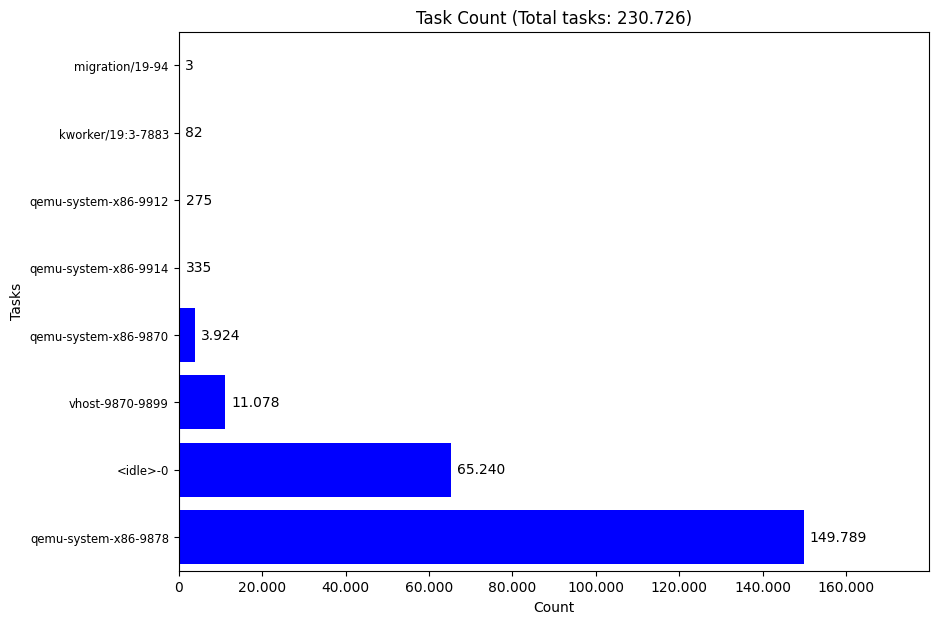
\includegraphics[width=1.0\columnwidth]{img/balanced/results_host_report.png}
		\caption[balanced host report]{balanced host report}
		\label{fig:balanced_kvm_host}
	\end{figure}
	\clearpage
	
	Figure~\ref{fig:balanced_kvm_guest} shows ...
	
	\begin{figure}[H]
		\centering
		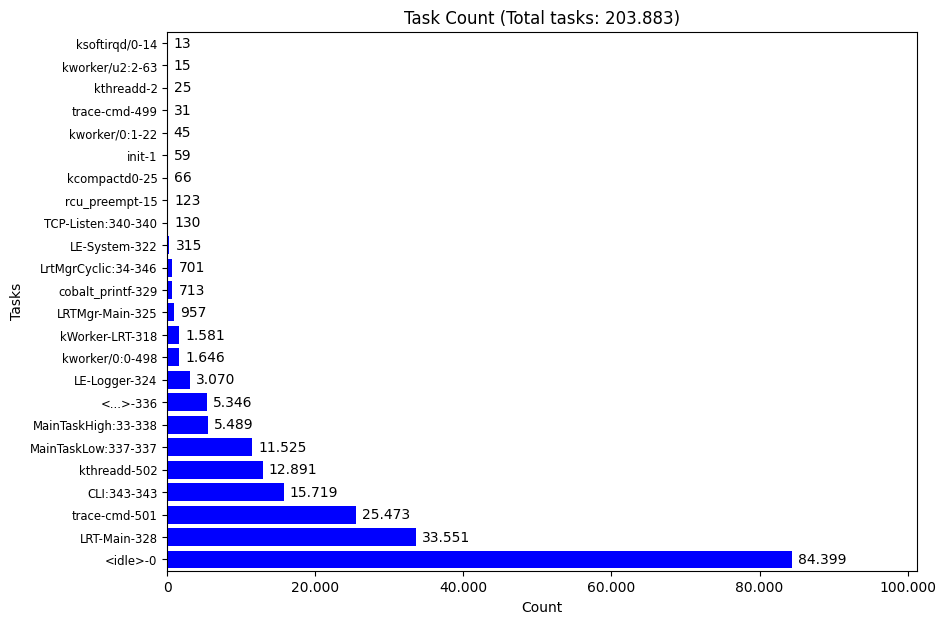
\includegraphics[width=1.0\columnwidth]{img/balanced/results_guest_report.png}
		\caption[balanced guest report]{balanced guest report}
		\label{fig:balanced_kvm_guest}
	\end{figure}
	\clearpage
	
	
	
	Figure~\ref{fig:performance_kvm_exit} shows ...
	
	\begin{figure}[H]
		\centering
		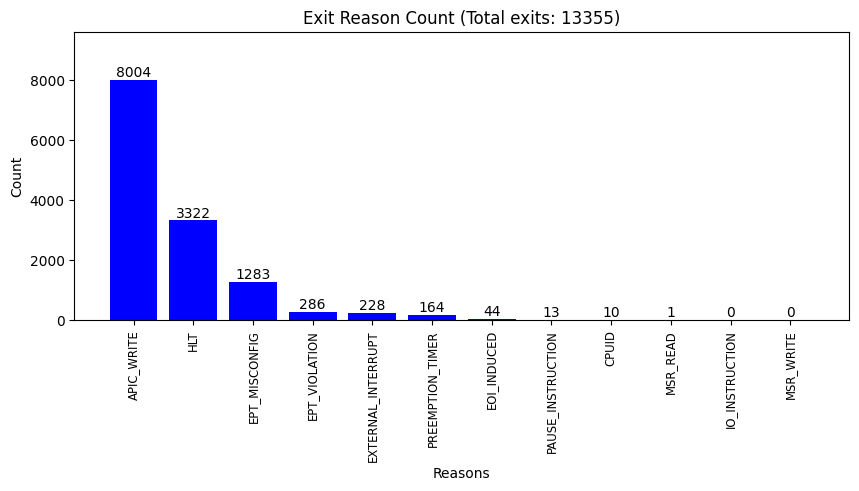
\includegraphics[width=1.0\columnwidth]{img/performance/kvm_exit_count.png}
		\caption[performance \_exit\_count]{performance \_exit\_count}
		\label{fig:performance_kvm_exit}
	\end{figure}
	\clearpage
	
	
	Figure~\ref{fig:performance_kvm_host} shows ...
	
	\begin{figure}[H]
		\centering
		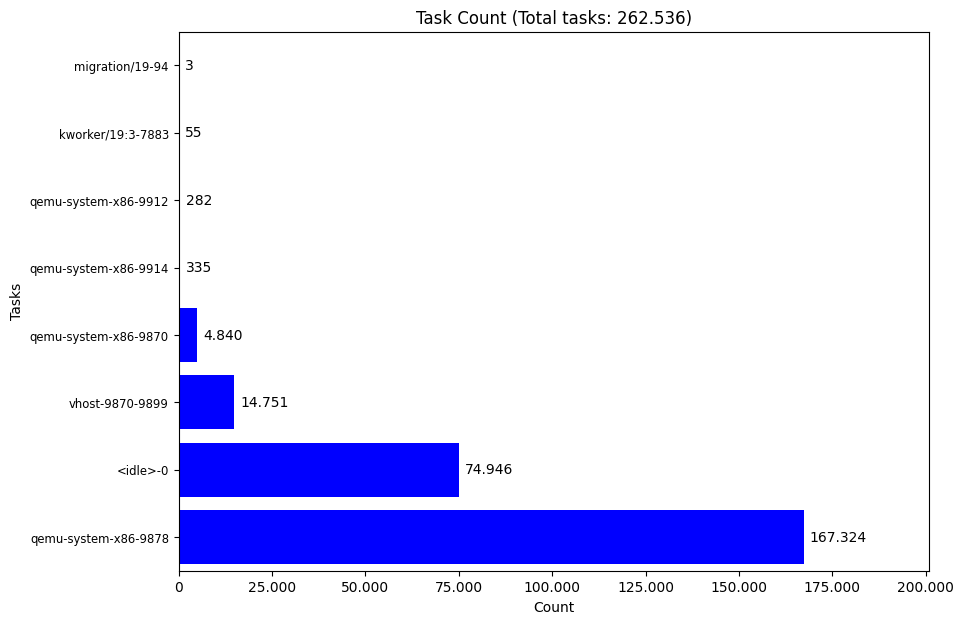
\includegraphics[width=1.0\columnwidth]{img/performance/results_host_report.png}
		\caption[performance host report]{performance host report}
		\label{fig:performance_kvm_host}
	\end{figure}
	\clearpage
	
	Figure~\ref{fig:performance_kvm_guest} shows ...
	
	\begin{figure}[H]
		\centering
		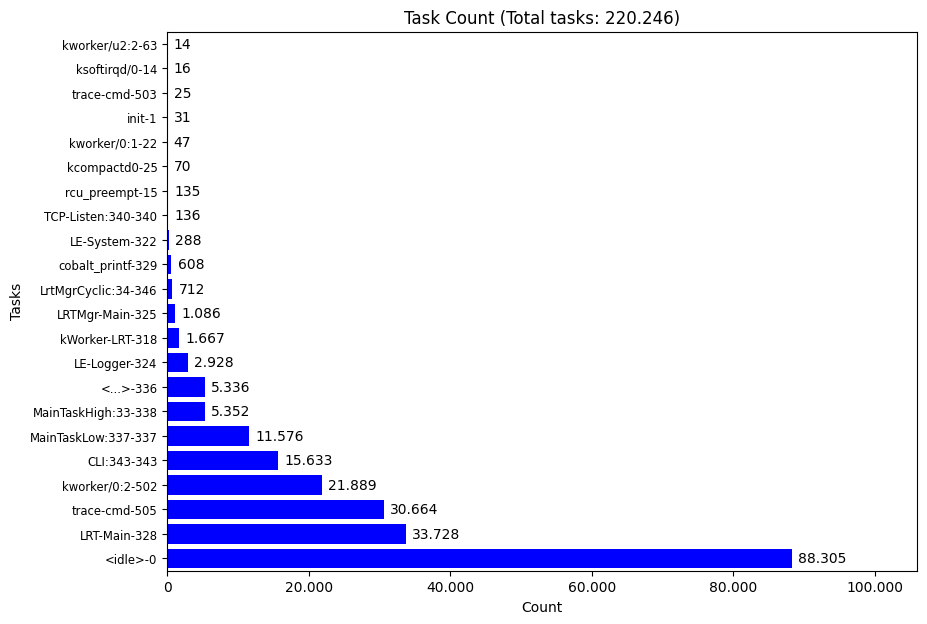
\includegraphics[width=1.0\columnwidth]{img/performance/results_guest_report.png}
		\caption[balanced guest report]{balanced guest report}
		\label{fig:performance_kvm_guest}
	\end{figure}
	\clearpage
	
	\noindent Without CPU isolation, context switches take place at operating system level and not at hypervisor level. This explains why there are fewer \texttt{kvm\_exit} events. However, this will also, as previously shown, lead to higher latency, as context switches at operating system level generally take longer than a \texttt{kvm\_exit} and kvm\_entry.
	
	\noindent When the CPU was dedicated to the QEMU process, on the other hand,there was a significant increase in \texttt{kvm\_exit} events. This is because every context switch takes place at hypervisor level. Nevertheless, lower latency was achieved thereby, as the qemu process is no longer influenced by the CPU scheduling of the operating system.
	
	Figure~\ref{fig:gnuplot_max_latency_default}
	\begin{figure}[H]
		\centering
		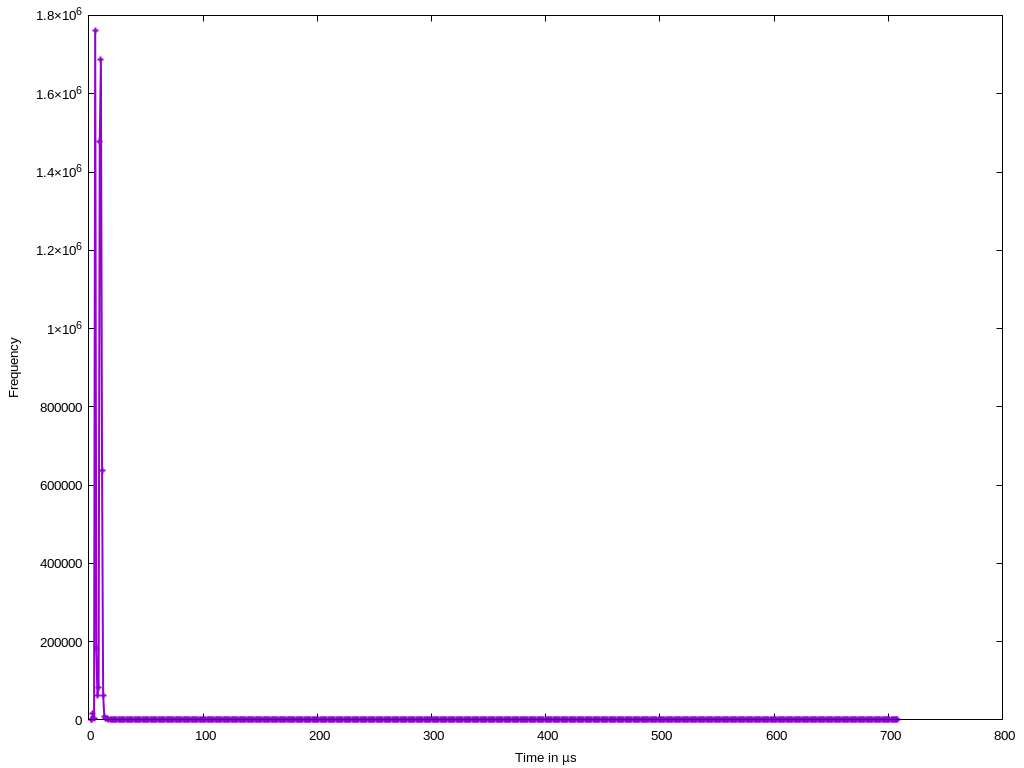
\includegraphics[width=0.8\columnwidth]{masterthesis-documentation/docs/sigmatek/xenomai/1default/gnuplot_max_latency_default.png}
		\caption[gnuplot latency no taskset]{gnuplot latency no taskset}
		\label{fig:gnuplot_max_latency_default}
	\end{figure}
	
	Figure~\ref{fig:gnuplot_max_latency_taskset}
	\begin{figure}[H]
		\centering
		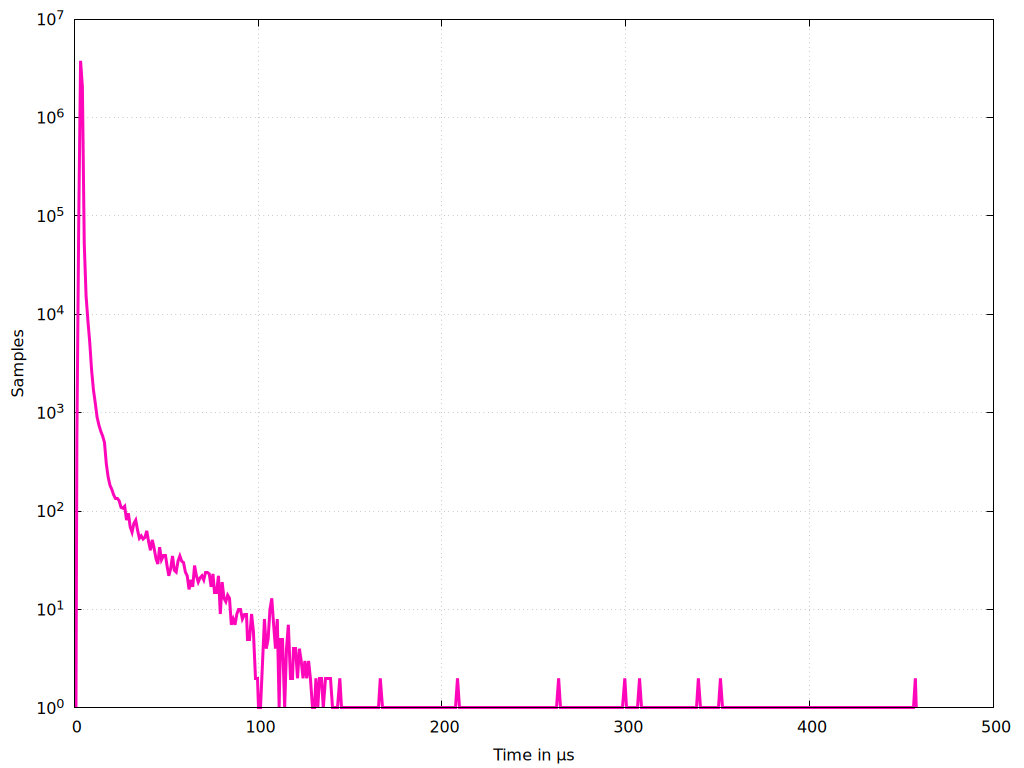
\includegraphics[width=0.8\columnwidth]{masterthesis-documentation/docs/sigmatek/xenomai/2taskset/gnuplot_max_latency_taskset.png}
		\caption[gnuplot latency with taskset]{gnuplot latency with taskset}
		\label{fig:gnuplot_max_latency_taskset}
	\end{figure}
	
	Figure~\ref{fig:gnuplot_max_latency_vapic}
	\begin{figure}[H]
		\centering
		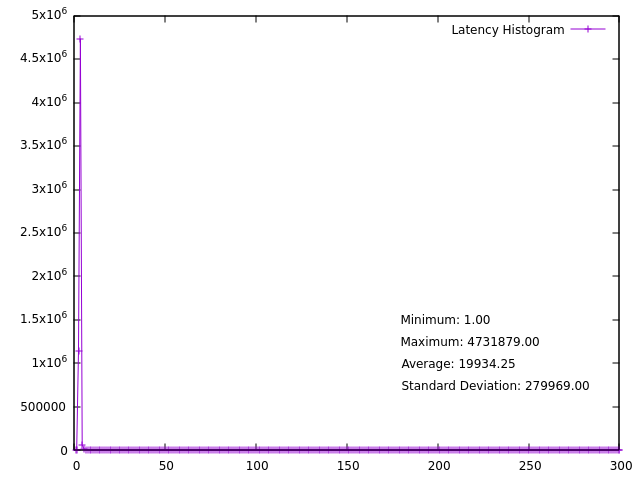
\includegraphics[width=0.8\columnwidth]{masterthesis-documentation/docs/sigmatek/xenomai/vapic/gnuplot_max_latency_vapic.png}
		\caption[gnuplot latency with taskset]{gnuplot latency with taskset}
		\label{fig:gnuplot_max_latency_vapic}
	\end{figure}

	\noindent In the process of analyzing the \texttt{kvm\_exit} events, several reasons for these exits were identified. The most frequent among these were the \texttt{APIC\_WRITE} and \texttt{HLT} events. The former is initiated when the guest writes to its Advanced Programmable Interrupt Controller (APIC), a component of the CPU that manages hardware interrupts. The latter occurs when the guest executes the HLT instruction, effectively halting the CPU until the next external interrupt is fired. Other significant but less frequent events included \texttt{EXTERNAL\_INTERRUPT} and \texttt{IO\_INSTRUCTION}. These events are indicative of the guest's interaction with hardware devices and its execution of I/O operations. Events such as \texttt{EPT\_MISCONFIG} and \texttt{PREEMPTION\_TIMER} were also noted. These could potentially signal issues with memory management and the host's scheduling of the guest. While events like \texttt{PAUSE\_INSTRUCTION}, \texttt{EPT\_VIOLATION}, \texttt{EOI\_INDUCED}, \texttt{MSR\_READ}, and \texttt{CPUID} were the least frequent, they still provide valuable insights into the guest's behavior and the host-guest interaction.

	The Advanced Programmable Interrupt Controller (APIC) is responsible for the distribution of interrupts in x86 and Itanium-based computer systems. An APIC\_WRITE occurs when a guest operating system attempts to write to the APIC registers. Since the APIC is a physical hardware component, KVM must intercept this operation and cause a VM exit. To avoid this, newer Intel processors offer hardware virtualization of the Advanced Programmable Interrupt Controller (APICv). APICv improves virtualized AMD64 and Intel 64 guest performance by allowing the guest to directly access the APIC, dramatically cutting down interrupt latencies and the number of virtual machine exits caused by the APIC. This feature is used by default in newer Intel processors and improves I/O performance. 

This can be done by setting the apic flag to 'v' in the VM configuration file.

Figure~\ref{fig:kvm_exit_vapic} shows \texttt{kvm\_exit} frequency with APIC virtualization. Comparing this to the previous Figures~\ref{fig:kvm_exit_taskset} and~\ref{fig:kvm_exits_default}, it can be observed that an APIC\_Write no longer occurs.


\begin{figure}[H]
	\centering
	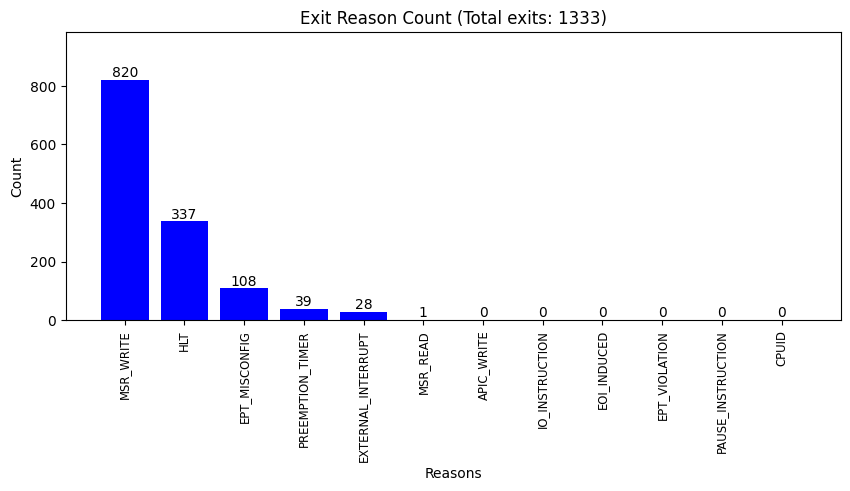
\includegraphics[width=1.0\columnwidth]{img/kvm_exit_vapic.png}
	\caption[kvm exits default]{kvm exits default}
	\label{fig:kvm_exit_vapic}
\end{figure}

\end{comment}

\chapter{Results}\label{cha:results}
~\cite{pixelartSIGMATEKKompletteAutomatisierungssysteme}
~\cite{Tracecmd}
~\cite{KernelShark}
~\cite{XenomaiXenomai}
~\cite{CPUEinheitenSIGMATEK}
~\cite{EngineeringToolLASAL}
~\cite{WelcomeYoctoProject}
~\cite{QEMU}
~\cite{maPerformanceTuningKVMbased}
~\cite{linPerformanceEvaluationXenomai}
~\cite{broskyShieldedProcessorsGuaranteeing2003}
~\cite{cinqueVirtualizingMixedCriticalitySystems2022}
~\cite{garcia-vallsChallengesRealtimeVirtualization2014}
~\cite{guStateoftheArtSurveyRealTime2012}
~\cite{HardRealTime}
~\cite{javierperezHowRealTime2022}
~\cite{kirovaImpactModernVirtualization2019}
~\cite{kiszkaLinuxRealTimeHypervisor}
~\cite{lutsykPipelinedMulticoreMachine2020}
~\cite{malallahComprehensiveStudyKernel2021}
~\cite{masrurVMBasedRealTimeServices2010}
~\cite{mckenneyRealTimeVs}
~\cite{pielAsymmetricSchedulingLoad2006}
~\cite{queirozTestingLimitsGeneralpurpose2023}
~\cite{reghenzaniRealTimeLinuxKernel2020}
~\cite{yoonRealTimePerformanceAnalysis}
~\cite{adamPerformanceAssessmentLinux2021}
~\cite{adamRealTimePerformanceResponse2021}
~\cite{deoliveiraDemystifyingRealTimeLinux}
~\cite{RealTimePerformanceTuning2022}
~\clearpage

\begin{comment}

VARAN-Bus PCV-521\newline
Windows\newline
Ubuntu\newline
WSL\newline\newline\newline



In Xenomai 3, you need:

The Linux kernel with the Dovetail interface, which allows the kernel to handle real-time tasks with low latency.
The Cobalt real-time core, which is responsible for scheduling and executing real-time tasks.
In Xenomai 4, you need:
The Linux kernel with the EVL interface, which, like Dovetail, enables the kernel to handle real-time tasks with low latency.
The libevl library, which provides a user interface to the EVL core, allowing applications to use the real-time capabilities provided by EVL.
So, while both versions require a Linux kernel with a real-time interface (Dovetail for Xenomai 3, EVL for Xenomai 4), Xenomai 3 uses a real-time core (Cobalt), while Xenomai 4 uses a library (libevl) to provide applications with access to its real-time capabilities.
\end{comment}
\clearpage

\chapter{Discussion}\label{cha:discussion}
\clearpage

\chapter{Summary and Outlook}\label{cha:summary_and_outlook}
%
% Hier beginnen die Verzeichnisse.
%
\clearpage
\printbibliography
\clearpage

% Das Abbildungsverzeichnis
\listoffigures
\clearpage

% Das Tabellenverzeichnis
\listoftables
\clearpage

% Das Quellcodeverzeichnis
\listofcode
\clearpage

\phantomsection
\addcontentsline{toc}{chapter}{\listacroname}

\chapter*{\listacroname}
\begin{acronym}[XXXXX]
	\acro{CPU}[CPU]{Central Processing Unit}
	\acro{QEMU}[QEMU]{Quick Emulator}
	\acro{IRQ}[IRQ]{Interrupt Request}
\end{acronym}

%
% Hier beginnt der Anhang.
%
\clearpage
\appendix

\chapter{Anhang A}
\clearpage

\chapter{Anhang B}

\end{document}
